
% \todoin{
% Main todos for appendix
% \begin{itemize}
%     \item describe which MI estimator is employed, how the data is sampled.
%     \item Train / test curves
%     \item Objectives combinations not discussed in main text
%     \item PPG without value distillation runs.
%     \item Analysis we have for sparsity, orthogonality, dynamics awareness metrics from https://arxiv.org/abs/2203.15955
% \end{itemize}
% }

\section{Theoretical results}\label{c2:app:proof}
\THGenBound*
\begin{proof}
    This result directly follows from a result obtained by \citet{instance_invariant} and reproduced below.
    \begin{theorem}
For any CMDP such that $|V^\pi (x)| \leq D/2,\forall x, \pi$, with $D$ being a constant, then for any set of training levels $L$, and policy $\pi$
\begin{equation}
    \E_{c\sim \mathcal{U}(L), x_0 \sim \mathcal{P}_0(c)}[V^\pi(x_0)] - \E_{c\sim P(\rc), x_0 \sim \mathcal{P}_0(c)}[V^\pi(x_0)] \leq \sqrt{\frac{2D^2}{|L|} \times \mut{\pi}{L}},
\end{equation}
\end{theorem}
Then, as $\pi \triangleq f \circ \phi_A$, by the data processing inequality we always have $\mut{\pi}{L} \leq \mut{Z_A}{L}$, and therefore,
\begin{align*}
    \E_{c\sim \mathcal{U}(L), x_0 \sim \mathcal{P}_0(c)}[V^\pi(x_0)] - \E_{c\sim P(\rc), x_0 \sim \mathcal{P}_0(c)}[V^\pi(x_0)] & \leq \sqrt{\frac{2D^2}{|L|} \times \mut{\pi}{L}}\\ 
& \leq \sqrt{\frac{2D^2}{|L|} \times \mut{Z_A}{L}}
\end{align*}.

\citet{garcin2024dred} follow the same reasoning and obtain an equivalent result, without restating the bound.

\end{proof}

\THmarkovmi*
\begin{proof}
This proof has two part. We first demonstrate that the Inverse Model condition of \Cref{c2:th:markov_z} from \citet{markov_z} (reproduced below) is satisfied if and only if $\mut{(Z,Z')}{A}=\mut{(X,X')}{A}$. We then show that if $\mut{Z}{Z'} =\mut{X}{X'}$ then the Density Ratio condition is also satisfied.
    \begin{theorem}\label{c2:th:markov_z}
    $\phi$ is a Markov representation if the following conditions hold for every timestep $t$ and any policy $\pi$:
    \begin{enumerate}
        \item \textbf{Inverse Model.} The inverse dynamic model, defined as $I(a|s',s)\coloneqq \frac{\mathcal{T}(s'|a,s)\pi(a|s)}{P^\pi(s'|s)}$, where $P^\pi(s'|s)=\sum_{\bar{a}\in\sA} \mathcal{T}(s'|\bar{a},s)\pi(a|s)$, should be equal in the original and reduced MDPs. That is we have $P^\pi(a|z',z)=P^\pi(a|s,s'), \forall a\in\sA, s,s'\in\sS$.
        \item \textbf{Density Ratio.} The original and abstract next-state density ratios are equal when conditioned on the same abstract state: $\frac{P^\pi(z'|z)}{P^\pi(z')}=\frac{P^\pi(s'|z)}{P^\pi(s')}, \forall x' \in \sS,$ where $P^\pi(s'|z)=\sum_{\bar{s}\in\sS} P^\pi(s'|\bar{s})\mu(\bar{s}|z)$ and $\mu(s|z) = \frac{\1_{\phi(s)=z} P^\pi(s)}{\sum_{\bar{s}\in\sS} P^\pi(s|\bar{s})}$. $P^\pi(s'|z)$ is the probability of transitioning to state $s'$ and $\mu(s|z)$ is the probability of currently being in state $s$ when in latent state $z$.
    \end{enumerate}
\end{theorem}

We begin with two observations that are useful for our derivation.

% Observation A: The causal interaction between $A$ and pairs $(X,X')$, $(O,O')$ and $(Z,Z')$ is described by the Markov Chain $A\leftrightarrow (X,X') \rightarrow (O,O') \rightarrow (Z,Z')$.

% Observation B: By inspection of the Markov chain above, we see that $(Z,Z')|A$ and $(X,X')|A$ are conditionally independent. Therefore we have 
% \begin{equation*}
%  p(a,z,z')=\sum_{x,x'\in X,X'} p(a,x,x')p(z,z'|x,x'), \forall a,z,z' \in  A ,  Z ,  Z'.
% \end{equation*}

Observation A: Given that any $z\in\sZ$ is obtained from the mapping $x \overset{\Omega}{\rightarrow} o \overset{\phi}{\rightarrow} z$, and that $h \triangleq \phi \circ \Omega$ is a deterministic (but not necessarily invertible) function, each element $x\in\sX$ maps to a single element $z\in\sZ$. It directly follows that $\forall a,z_1,z_2 \in \sA\times\sZ\times \sZ$, we have
\begin{equation*}
    p(a,z_1, z_2) = \sum_{x_1,x_2\in \sX^2} p(a,x_1,x_2) \1[z_1,z_2=h(x_1),h(x_2)]
\end{equation*}
and
\begin{equation*}
    p(z_1, z_2) = \sum_{x_1,x_2\in \sX^2} p(x_1,x_2) \1[z_1,z_2=h(x_1),h(x_2)]
\end{equation*}
Observation B: Let $P^{\pi}(a,x,x')$ be the joint distribution of elements in $(A,X,X')$ collected under policy $\pi$, we have $P^{\pi}(a,x_1,x_2)>0$ if and only if $a,x_1,x_2 \in (A,X,X')$.

Observation C: Similarly to obs. B, we have $P^{\pi}(x_1,x_2)>0$ if and only if $x_1,x_2 \in (X,X')$.
% \begin{equation*}
%     p(\bar{z},\bar{z}'|x,x') = 
%     \begin{cases}
%         1& \text{ if } \bar{z},\bar{z}'=z,z'\\
%         0& \text{ otherwise }
%     \end{cases}
% \end{equation*}


1) \textit{Proving that the Inverse Model condition is satisfied if and only if} $\mut{(Z,Z')}{A}=\mut{(X,X')}{A}$.

The above is equivalent to showing that the Inverse Model condition is satisfied if and only if $\entropy (A|Z,Z') = \entropy (A|X,X')$. For $\entropy (A|Z,Z')$, we have
\begin{align*}
    \entropy (A|Z,Z') &= -\sum_{A  ,  Z  ,  Z'} P^\pi(a,z,z') \log P^\pi(a|z,z') \\
    \text{(from obs. A)} \quad    &= -\sum_{\sA \times\sZ\times\sZ} \sum_{x_1,x_2\in \sX^2} P^\pi(a,x_1,x_2) \1[z,z'=h(x_1),h(x_2)]  \log P^\pi(a|z,z')\\
   \text{(from obs. B)} \quad & = -\sum_{\sA \times\sX\times\sX} P^\pi (a,x,x')\sum_{\sZ^2}\1[z,z'=h(x),h(x')]\log P^\pi (a|z,z') \\
        % & = -\sum_{A  ,  X  ,  X'}P^\pi (a,x,x')\sum_{\sZ^2}\1[z,z'=h(x),h(x')]\log P^\pi (a|z,z')  \\
    & = - \sum_{\sA \times\sX\times\sX} P^\pi (a,x,x') \log \prod_{\sZ^2} P^\pi (a|z,z')^{\1[z,z'=h(x),h(x')]}\\
    & = - \sum_{\sA \times\sX\times\sX} P^\pi (x,x')P^\pi (a|x,x') \log \prod_{\sZ^2} P^\pi (a|z,z')^{\1[z,z'=h(x),h(x')]}\\
    & = - \E_{X  ,  X'} [\sum_\sA P^\pi (a|x,x') \log \prod_{\sZ^2} P^\pi (a|z,z')^{\1[z,z'=h(x),h(x')]}]
\end{align*}
It follows that 
\begin{align*}
    \entropy (A|Z,Z') - \entropy (A|X,X') &=\E_{X  ,  X'}\bigg[\sum_\sA P^\pi (a|x,x') \log \frac{P^\pi (a|x,x')}{\prod_{\sZ^2} P^\pi (a|z,z')^{\1[z,z'=h(x),h(x')]}}\bigg] \\
    & = \E_{X,X'}[ \KL (P \Vert Q)],
    % & = \E_{X,X'}[ \KL (P^\pi (a|x,x') \Vert \prod_{z,z'\in  Z^2} P^\pi (z,z'|x,x') P^\pi (a|z,z'))]
\end{align*}
with $P=P^\pi (a|x,x')$ and $Q=\prod_{z,z'\in  Z,Z'} P^\pi (a|z,z')^{\1[z,z'=h(x),h(x')]}$. From Gibbs inequality we always have $\KL (p \Vert q) \geq 0$, therefore $\mut{(Z,Z')}{A}=\mut{(X,X')}{A}$ if and only if $\KL (P \Vert Q) = 0$  $\forall x,x' \in X,X'$, which is the case if and only if $P=Q$ almost $\mu$-everywhere.

From observation A, any $x_1,x_2\in \sX^2$  maps to exactly one pair $z_1,z_2\in\sZ^2$, and by construction of $X,X',Z,Z'$, for any pair $x,x'\in X,X'$, we must have $Q=\prod_{\bar{z},\bar{z}'\in  \sZ^2}P^\pi(a|\bar{z},\bar{z}')^{\1[\bar{z},\bar{z}'=h(x),h(x')]}=P^\pi (a|z,z')$, with $z,z'$ being the corresponding pair in $Z,Z'$.

Therefore $\mut{(Z,Z')}{A}=\mut{(X,X')}{A}$ if and only if $P^\pi (a|x,x')=P^\pi (a|z,z') \forall x,x',z,z'\in X,X',Z,Z'$, and we recover the Inverse Model condition.

Conversely, if the Inverse Model condition is not satisfied, then $\exists x,x',z,z',a\in X,X',Z,Z',A$ for which $P\neq Q$. Then $\KL (P \Vert Q)>0$ at $x,x'$ and $\mut{(Z,Z')}{A}<\mut{(X,X')}{A}$. 

2) \textit{Proving that the Density Ratio condition is satisfied if} $\mut{Z}{Z'}=\mut{X}{X'}$.

We first show that satisfying 
\begin{equation}\label{c2:eq:sufficient_cond_density_ratio}
    \frac{P^\pi(x'|x)}{P^\pi(x')}=\frac{P^\pi(z'|z)}{P^\pi(z')} \quad \forall x,x',z,z'\in X,X',Z,Z'
\end{equation}
is sufficient for satisfying the Density Ratio condition $\frac{P^\pi(x'|z)}{P^\pi(x')}=\frac{P^\pi(z'|z)}{P^\pi(z')}$. We then show that the condition in \Cref{c2:eq:sufficient_cond_density_ratio} holds if and only if $\mut{Z}{Z'}=\mut{X}{X'}$.

i) \textit{Showing the Density Ratio condition holds when  \Cref{c2:eq:sufficient_cond_density_ratio} is satisfied.}
First we notice that, $\forall x',z \in X',Z$, we have
\begin{equation*}
    P^\pi(x'|z) = \sum_{\bar{x}\in \sX} \1[z=h(\bar{x})]P^\pi(x'|\bar{x}) = \E_X [P^\pi(x'|x)].
\end{equation*}
Then, supposing \Cref{c2:eq:sufficient_cond_density_ratio} holds, we must have
\begin{equation*}
   P^\pi(x'|z) = \E_X [P^\pi(x'|x)] = P^\pi(x') \frac{P^\pi(z'|z)}{P^\pi(z')} \quad \forall x',z,z'\in X',Z,Z',
\end{equation*}
and the Density Ratio condition holds.

ii) \textit{Proving \Cref{c2:eq:sufficient_cond_density_ratio} holds if and only if} $\mut{Z}{Z'}=\mut{X}{X'}$.

We have
\begin{align*}
\mut{Z}{Z'} &= \sum_{\sZ^2} P^\pi (z,z') \log\frac{P^\pi(z'|z)}{P^\pi(z')}\\
\text{(from obs. A)} \quad  &=  \sum_{\sZ^2} \sum_{x_1,x_2\in \sX^2}  P^\pi (x_1,x_2) \1[z,z'=h(x_1),h(x_2)] \log\frac{P^\pi(z'|z)}{P^\pi(z')}\\
\text{(from obs. C)} \quad &= \sum_{\sX^2} P^\pi (x,x') \sum_{\sZ^2} \1[z,z'=h(x),h(x')] \log\frac{P^\pi(z'|z)}{P^\pi(z')}\\
&= \E_{X,X'} \bigg[\log \prod_{\sZ^2} \bigg(\frac{P^\pi(z'|z)}{P^\pi(z')}\bigg)^{\1[z,z'=h(x),h(x')]}\bigg].
\end{align*}
Then,
\begin{equation*}
    \mut{X}{X'}- \mut{Z}{Z'} = \E_{X,X'}[ \KL (P' \Vert Q')],
    % & = \E_{X,X'}[ \KL (P^\pi (a|x,x') \Vert \prod_{z,z'\in  Z^2} P^\pi (z,z'|x,x') P^\pi (a|z,z'))]
\end{equation*}
with
\begin{equation*}
    P'=\frac{P^\pi(x'|x)}{P^\pi(x')} \quad \text{and} \quad Q=\prod_{\sZ^2}\bigg(\frac{P^\pi(z'|z)}{P^\pi(z')}\bigg)^{\1[z,z'=h(x),h(x')]}
\end{equation*}
The remainder of this part follows the same structure as for the first part of the proof. 

$\mut{X}{X'}=\mut{Z}{Z'}$ if and only if  $\forall x,x' \in X,X'$, $P=Q$ almost $\mu$-everywhere. Any $x_1,x_2\in \sX^2$  maps to exactly one pair $z_1,z_2\in\sZ^2$, and by construction of $X,X',Z,Z'$, for any pair $x,x'\in X,X'$, we must have 
\begin{equation*}
    Q=\prod_{\bar{z},\bar{z}'\in\sZ^2}\bigg(\frac{P^\pi(\bar{z}'|\bar{z})}{P^\pi(\bar{z}')}\bigg)^{\1[\bar{z},\bar{z}'=h(x),h(x')]} = \frac{P^\pi(z'|z)}{P^\pi(z')},
\end{equation*}
with $z,z'$ being the corresponding pair in $Z,Z'$.

Therefore $\mut{X}{X'} = \mut{Z}{Z'}$ if and only if $\forall x,x',z,z'\in X,X',Z,Z'$ we have $\frac{P^\pi(x'|x)}{P^\pi(x')}=\frac{P^\pi(z'|z)}{P^\pi(z')}$. Finally, from i) being true, the Density ratio condition must hold.
\end{proof}


\LEMmiZLcond*
\begin{proof}
    Given $\pi$ is fixed while the batch $O$ is collected, for a single batch the causal interaction between $L$, $O$ and $Z$ is described by the Markov chain $X \rightarrow O \rightarrow Z$, where $x=(s,\lvl) \in \sS \times L$ and isn't directly observed. By the data processing inequality, $\mut{L}{Z} \leq \mut{L}{O}$, and as such $\mut{L}{O}>0$ is a necessary condition for $\mut{L}{Z}$ to be positive.

    Note that
    \begin{equation*}
        \mut{L}{Z} = \entropy(L) + \entropy(Z) - \entropy(L,Z) = 0 \Leftrightarrow \entropy(L,Z) = \entropy(L) + \entropy(Z),
    \end{equation*}
    that is, if and only if $Z$ and $L$ are independently distributed. Given the causal relationship between $L$ and $Z$, $\mu(z|\lvl)$ is well defined $\forall z,\lvl \in Z\times L$. If $\exists z_k,\lvl_j \in Z\times L$ such that $\mu(z_k|\lvl_j) \neq \mu(z_k)$ then $Z$ and $L$ cannot be independently distributed, and $\mut{L}{Z}>0$.
\end{proof}

\LEMmiZZandZL*
\begin{proof}
    
    Proof for condition a) : By the causal structure $V \leftarrow X \rightarrow O \rightarrow Z$ and the chain rule of mutual information, we have
    \begin{equation*}
    \mut{Z}{L} = \mut{Z}{V} - \mut{Z}{V|L} + \mut{Z}{L|V},
    \end{equation*}

    $\mut{Z}{L|V}$ is the information encoded in $Z$ about the training levels that does not depend on $V$. $\mut{Z}{V} - \mut{Z}{V|L}$ represents the information encoded in $Z$ about state values that is level-specific. If this term increases then $\mut{Z}{L}$ will also increase.

    Proof for condition b) : Consider an episode of arbitrary length $N$ collected with policy $\pi$. We depict the causal structure that exists between elements in the top row of \Cref{c2:fig:lemZZandZL} (elements may be repeated within each sequence). It naturally follows that we have the causal structure depicted in the bottom row when considering all levels in $L$. By the chain rule of mutual information, we have
    \begin{equation*}
        \mut{Z}{L} = \mut{Z}{(Z',L)} - \mut{Z}{Z'|L} = \mut{Z}{L|Z'} + \mut{Z}{Z'} - \mut{Z}{Z'|L},
    \end{equation*}
    and it follows that $\mut{Z}{L}$ increases with $\mut{Z}{Z'} - \mut{Z}{Z'|L}$. 
    
\end{proof}

% \begin{restatable}{lemma}{LEMmiZV}\label{c2:lem:miZV}
%     $\mut{Z}{V} > 0$ if $\mut{O}{V}>0$ and $\exists z_k,v_m \in Z\times V$ such that $\frac{1}{L} \sum_{\lvl \in L} p(z_k,v_m|\lvl) \neq p(z_k)p(v_m)$.
% \end{restatable}
% \begin{proof}
%     For a fixed policy $\pi$, state values are determined by $V^\pi(x)$, where $x=(s,\lvl) \in \sS \times L$. We then have the causal structure $V \leftarrow X \rightarrow O \rightarrow Z$, with no direct causal link between $Z$ and $V$. By the data processing inequality, $\mut{Z}{V} \leq \mut{O}{V}$, and as such $\mut{O}{V}>0$ is a necessary condition for $\mut{Z}{V}$ to be positive.

%     We have $\mut{Z}{V}=0$ if and only if $Z$ and $V$ are independently distributed. If $\frac{1}{L} \sum_{\lvl \in L}p(z_k,v_m|\lvl) \neq p(z_k)p(v_m)$ for some $z_k,v_m \in Z\times V$, then $p(z,v)=\frac{1}{L} \sum_{\lvl \in L} p(z,v|\lvl)\neq p(z)p(v)$ and $Z$ and $V$ cannot be independent.

% \end{proof}

\begin{figure}
\centering
    \begin{subfigure}[]{0.49\linewidth}
    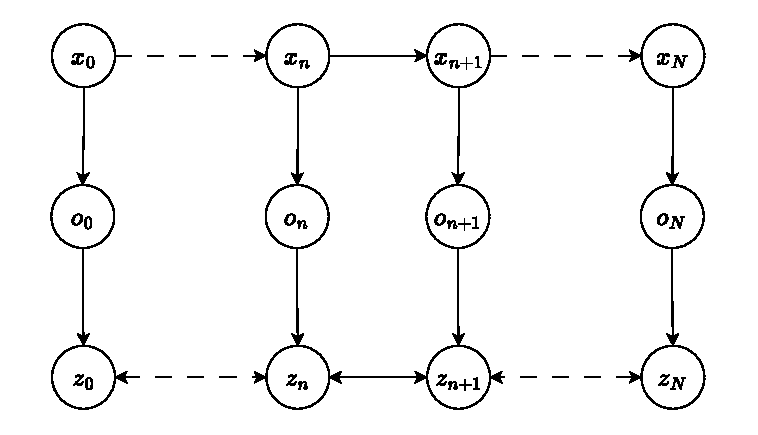
\includegraphics[width=1\linewidth]{supp/o_sequence.pdf}
    \end{subfigure}
    \begin{subfigure}[]{0.49\linewidth}
    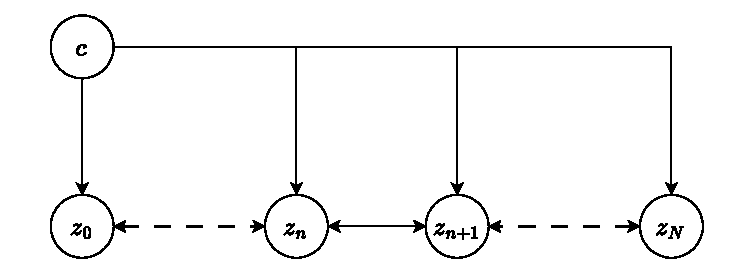
\includegraphics[width=1\linewidth]{supp/z_sequence.pdf}
    \end{subfigure}\\
    \begin{subfigure}[]{0.37\linewidth}
    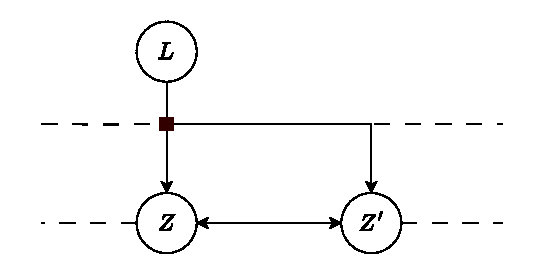
\includegraphics[width=1\linewidth]{supp/causalLZZ.pdf}
    \end{subfigure}
    \caption{In the top row, left, we depict the causal graph of states, observation and latents obtained over an episode. On the same row we draw a simplified graph that focuses on the relationship between $c$ and $Z_{0:N}$, and utilises the notion that the context remains the same throughout the episode. In the bottom row we draw the resulting causal relationship between $L$, $Z$ and $Z'$.}
    \label{c2:fig:lemZZandZL}
\end{figure}

% \begin{restatable}{corollary}{LEMmiZZA}\label{c2:lem:miZZA}
%    $\mut{(Z;Z')}{A}$ can still be positive when $(Z,Z')|L$ and $A|L$ are conditionally independent. %That is $p(z_m,v_k|\lvl) = p(z_m|\lvl)p(v_k|\lvl) \forall z_k,v_m,\lvl \in Z\times V \times L$. 
%     If $\mut{(Z;Z')}{A} > 0$ and $(Z,Z')|L$, $A|L$ are conditionally independent, then \{$\mut{Z}{L} > 0$ and $\mut{A}{L} >0$\} and/or \{$\mut{Z'}{L} > 0$ and $\mut{A}{L} > 0$\}.
% % either of the following conditions are met:
% % \begin{equation*}
% % \mut{Z}{L} > 0 \text{ and }\mut{A}{L} >0 \qquad
% % \mut{Z'}{L} > 0 \text{ and } \mut{A}{L} > 0.
% % \end{equation*}
% \end{restatable}
% \begin{proof}
%     $\mut{(Z,Z')}{A} \geq \max (\mut{Z}{A}, \mut{Z'}{A})$, therefore showing that either is $\mut{Z}{A}$ or $\mut{Z'}{A}$ is positive is sufficient. 
    
%     The rest of the proof directly follows the proof for \Cref{c2:cor:miZV}. We will have $\mut{Z}{A}>0$, $\mut{Z}{L}>0$ and $\mut{A}{L}>0$ given the causal chain $A \leftarrow X \rightarrow O \rightarrow Z$, even under conditional independence between $Z|L$ and $A|L$. Similarly, we will have $\mut{Z'}{A}>0$, $\mut{Z'}{L}>0$ and $\mut{A}{L}>0$ given the causal chain $A \leftarrow X' \rightarrow O' \rightarrow Z'$.
% \end{proof}

%TODO: removing from now, add in prep for rebuttals?
% \section{Mathematical workings for example in \Cref{c2:sec:toy_ex}}\label{c2:app:toy_ex_math}

\newpage
\section{Additional Figures and Tables}\label{c2:app:additional-plots}

\begin{figure}[!h]
    \begin{center}
    \centering
    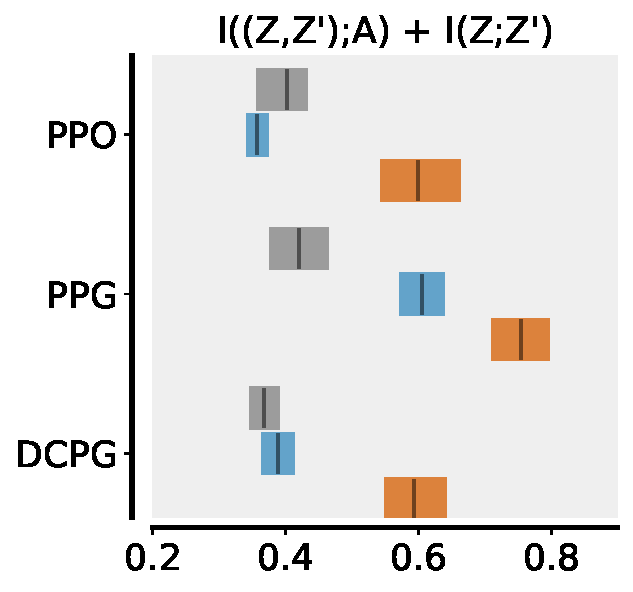
\includegraphics[width=0.3\textwidth]{figs/procgen_added.pdf}
    \end{center}
    \caption{$I((Z,Z^{\prime});A) + I(Z;Z^{\prime})$ for shared (gray), actor (blue) and critic (orange) for PPO, PPG, and DCPG in Procgen.}
    \label{c2:fig:mi_sum_markov}
\end{figure}

\begin{figure}[!h]
    \begin{center}
    \centering
    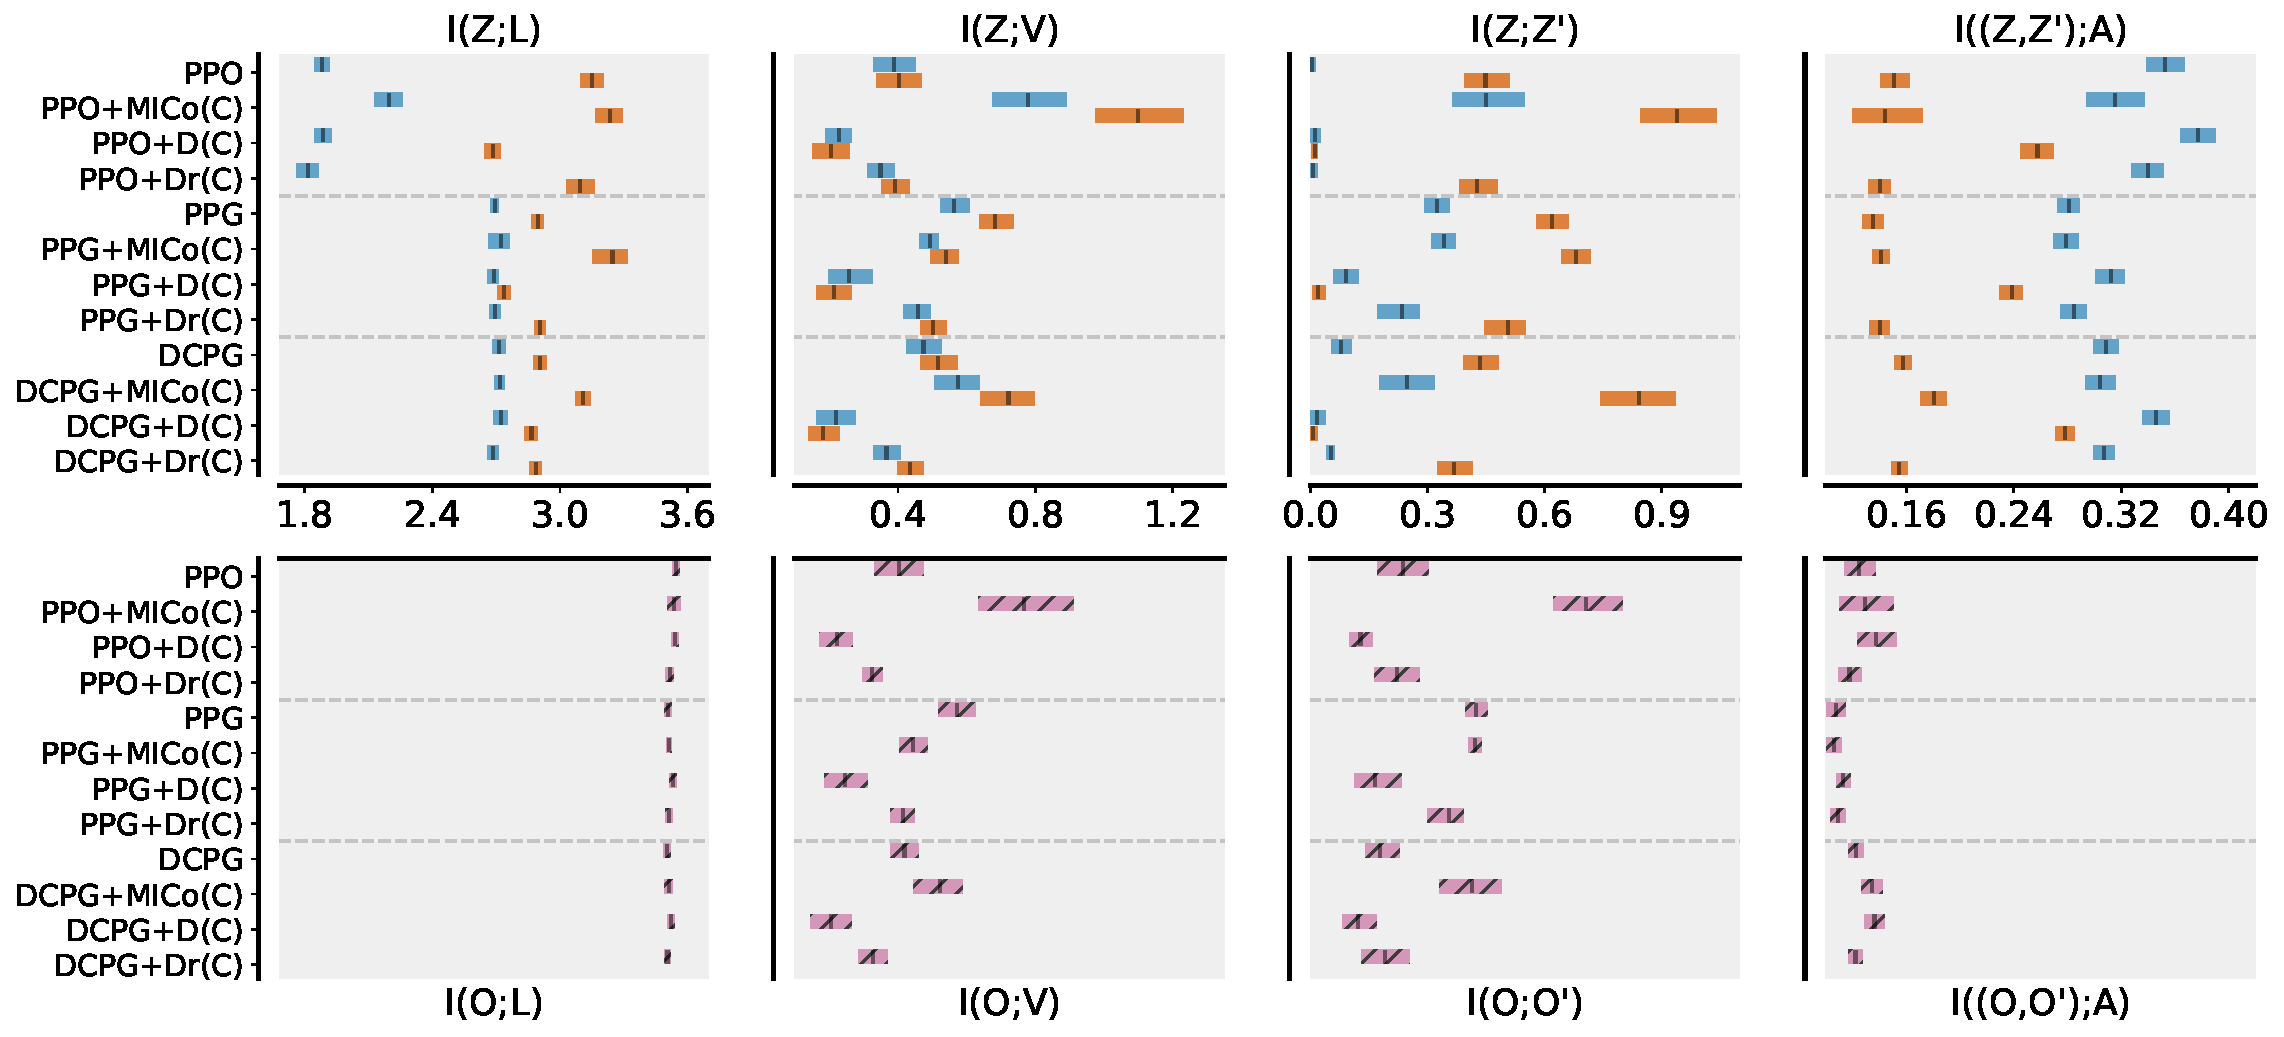
\includegraphics[width=0.97\textwidth]{figs/procgen_critic_algos_mi_tworow.pdf}
    \end{center}
    \caption{Mutual information measurements for the actor (blue) and critic (orange) for auxiliary losses applied to the critic for PPO, PPG, and DCPG in Procgen. Top/bottom rows are $I(Z;\cdot)$/$I(O;\cdot)$ with a shared x-axis.}
    \label{c2:fig:critic_objs}
\end{figure}

\begin{figure}[!h]
    \begin{center}
    \centering
    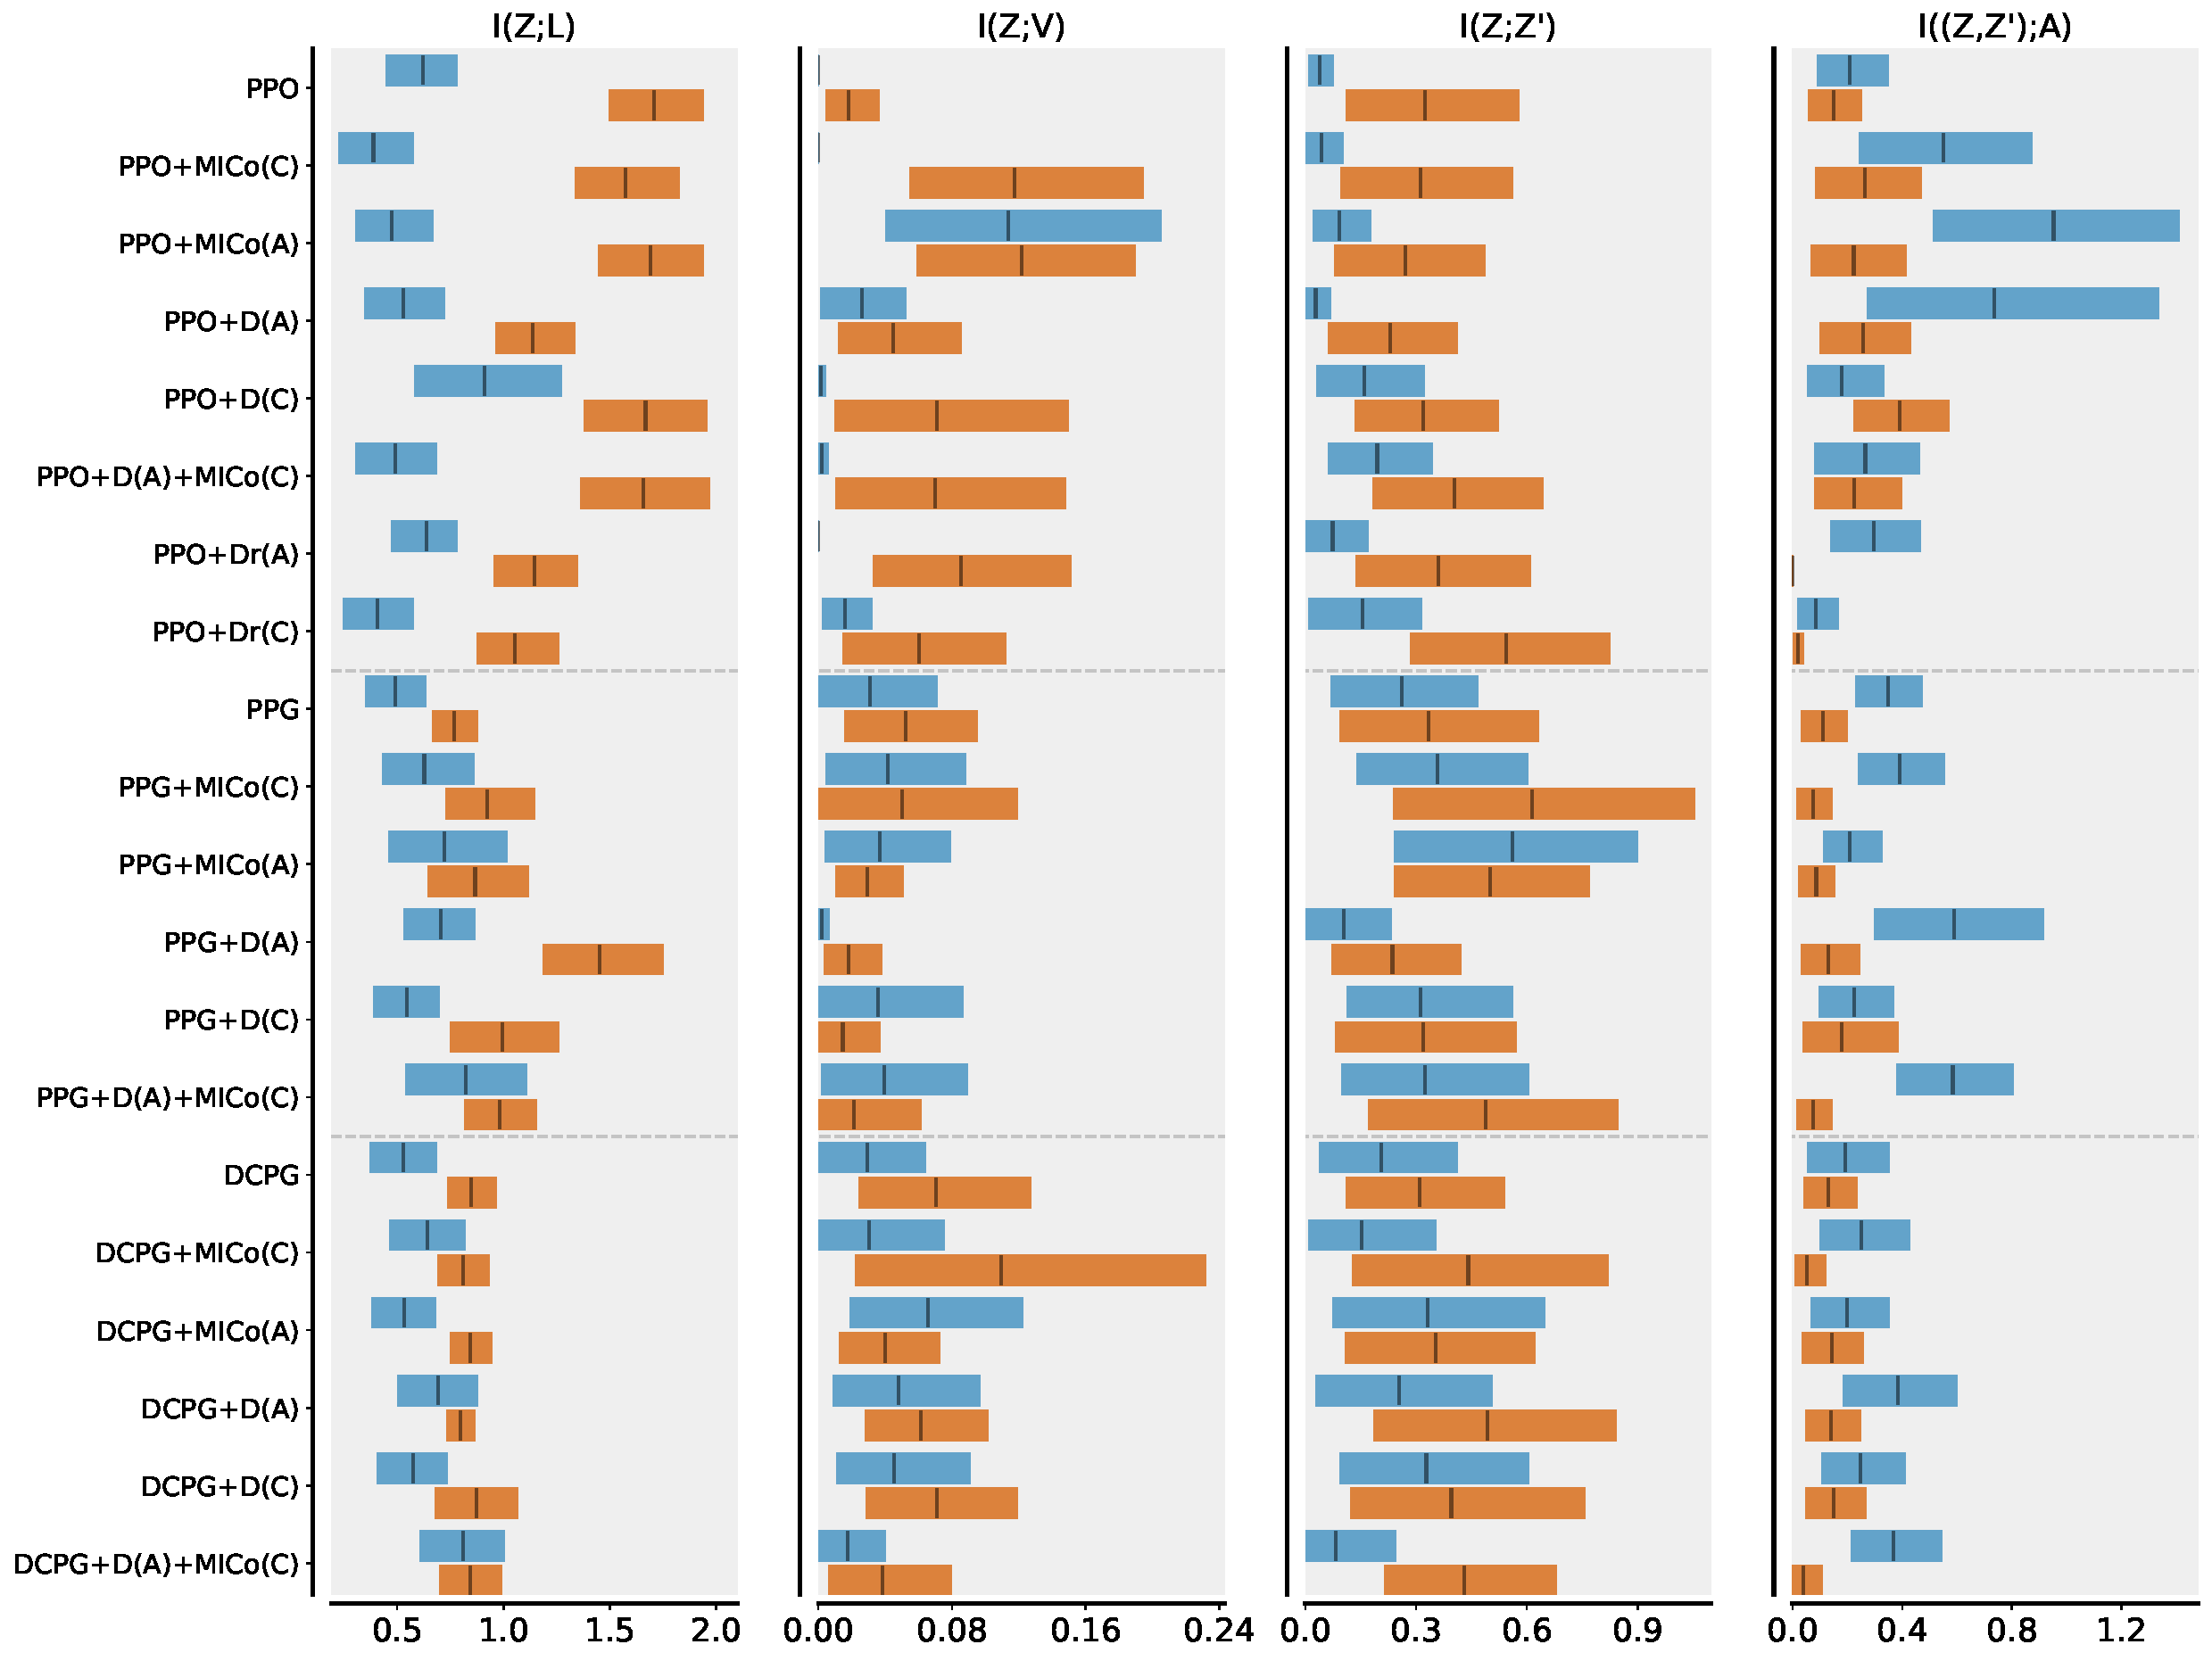
\includegraphics[width=0.97\textwidth]{figs/procgen_all_algos_mi.pdf}
    \end{center}
    \caption{$I(Z;\cdot)$ measurements for the actor (blue) and critic (orange) for auxiliary losses for PPO, PPG, and DCPG in Procgen.}
    \label{c2:fig:procgen_all_miZ}
\end{figure}

\begin{figure}[!h]
    \begin{center}
    \centering
    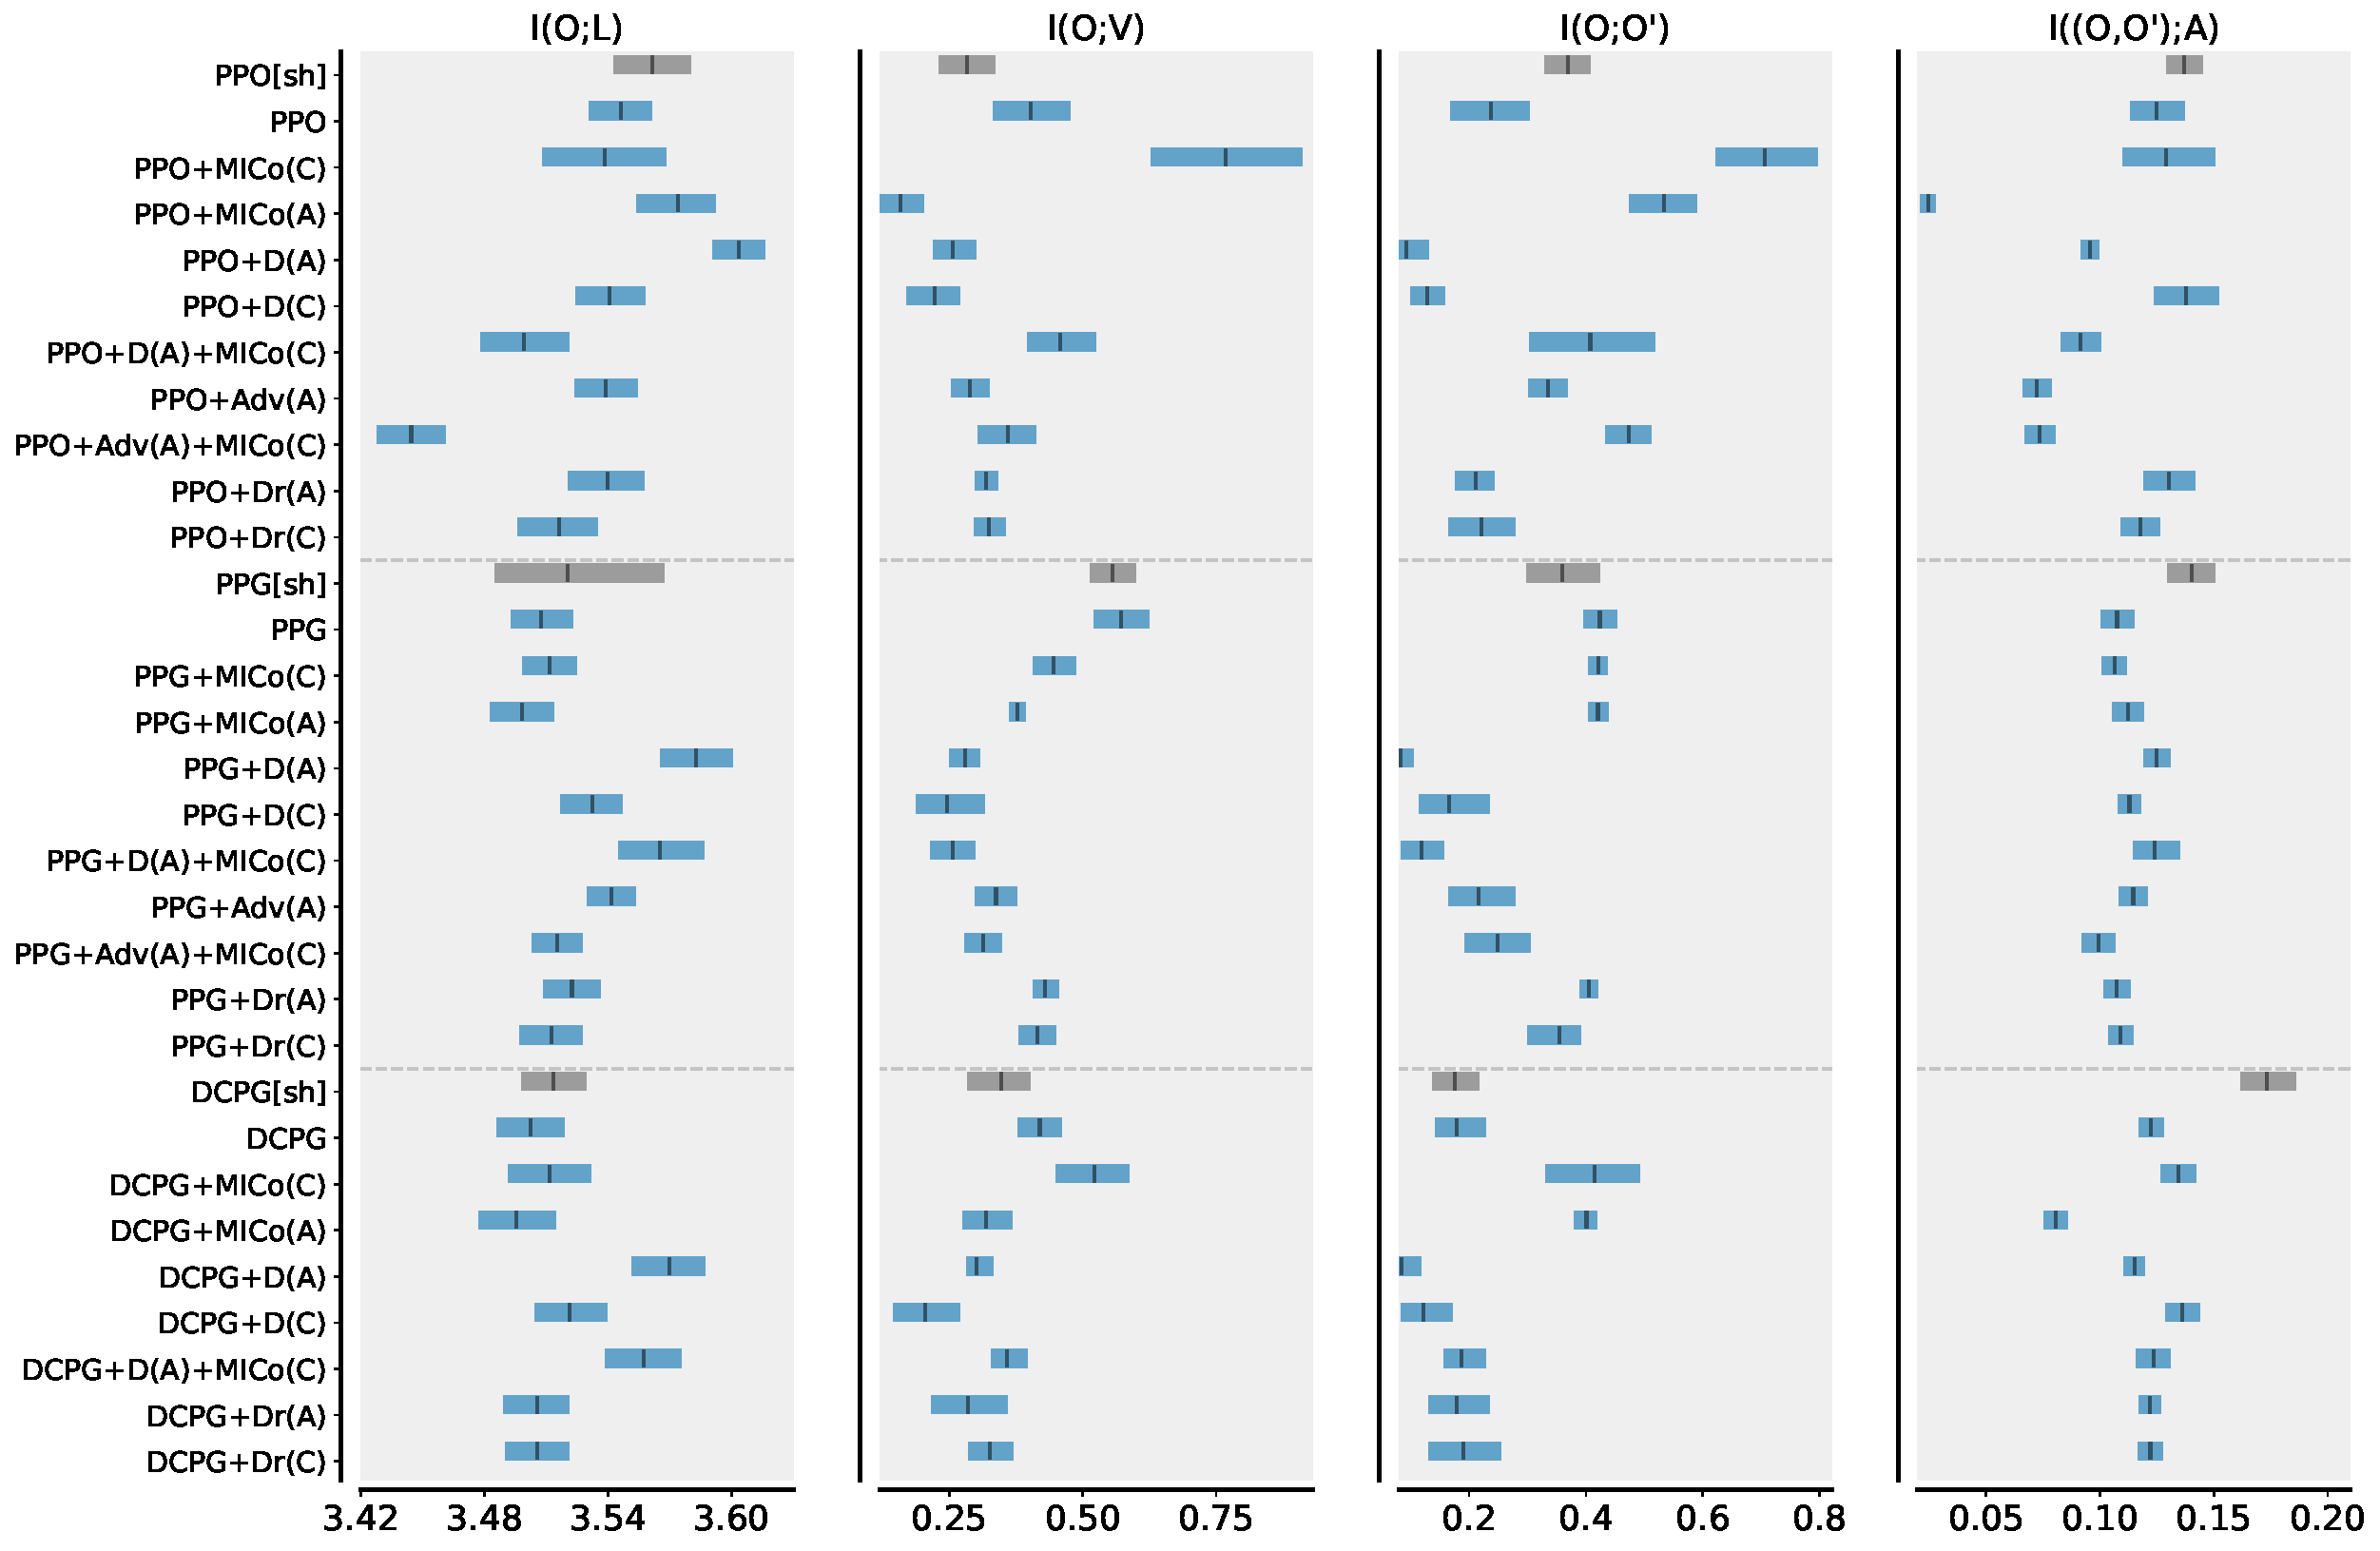
\includegraphics[width=0.97\textwidth]{figs/procgen_all_algos_miO.pdf}
    \end{center}
    \caption{$I(O;\cdot)$ measurements for the actor (blue) and critic (orange) for auxiliary losses for PPO, PPG, and DCPG in Procgen.}
    \label{c2:fig:procgen_all_miO}
\end{figure}

\begin{figure}[!h]
    \begin{center}
    \centering
    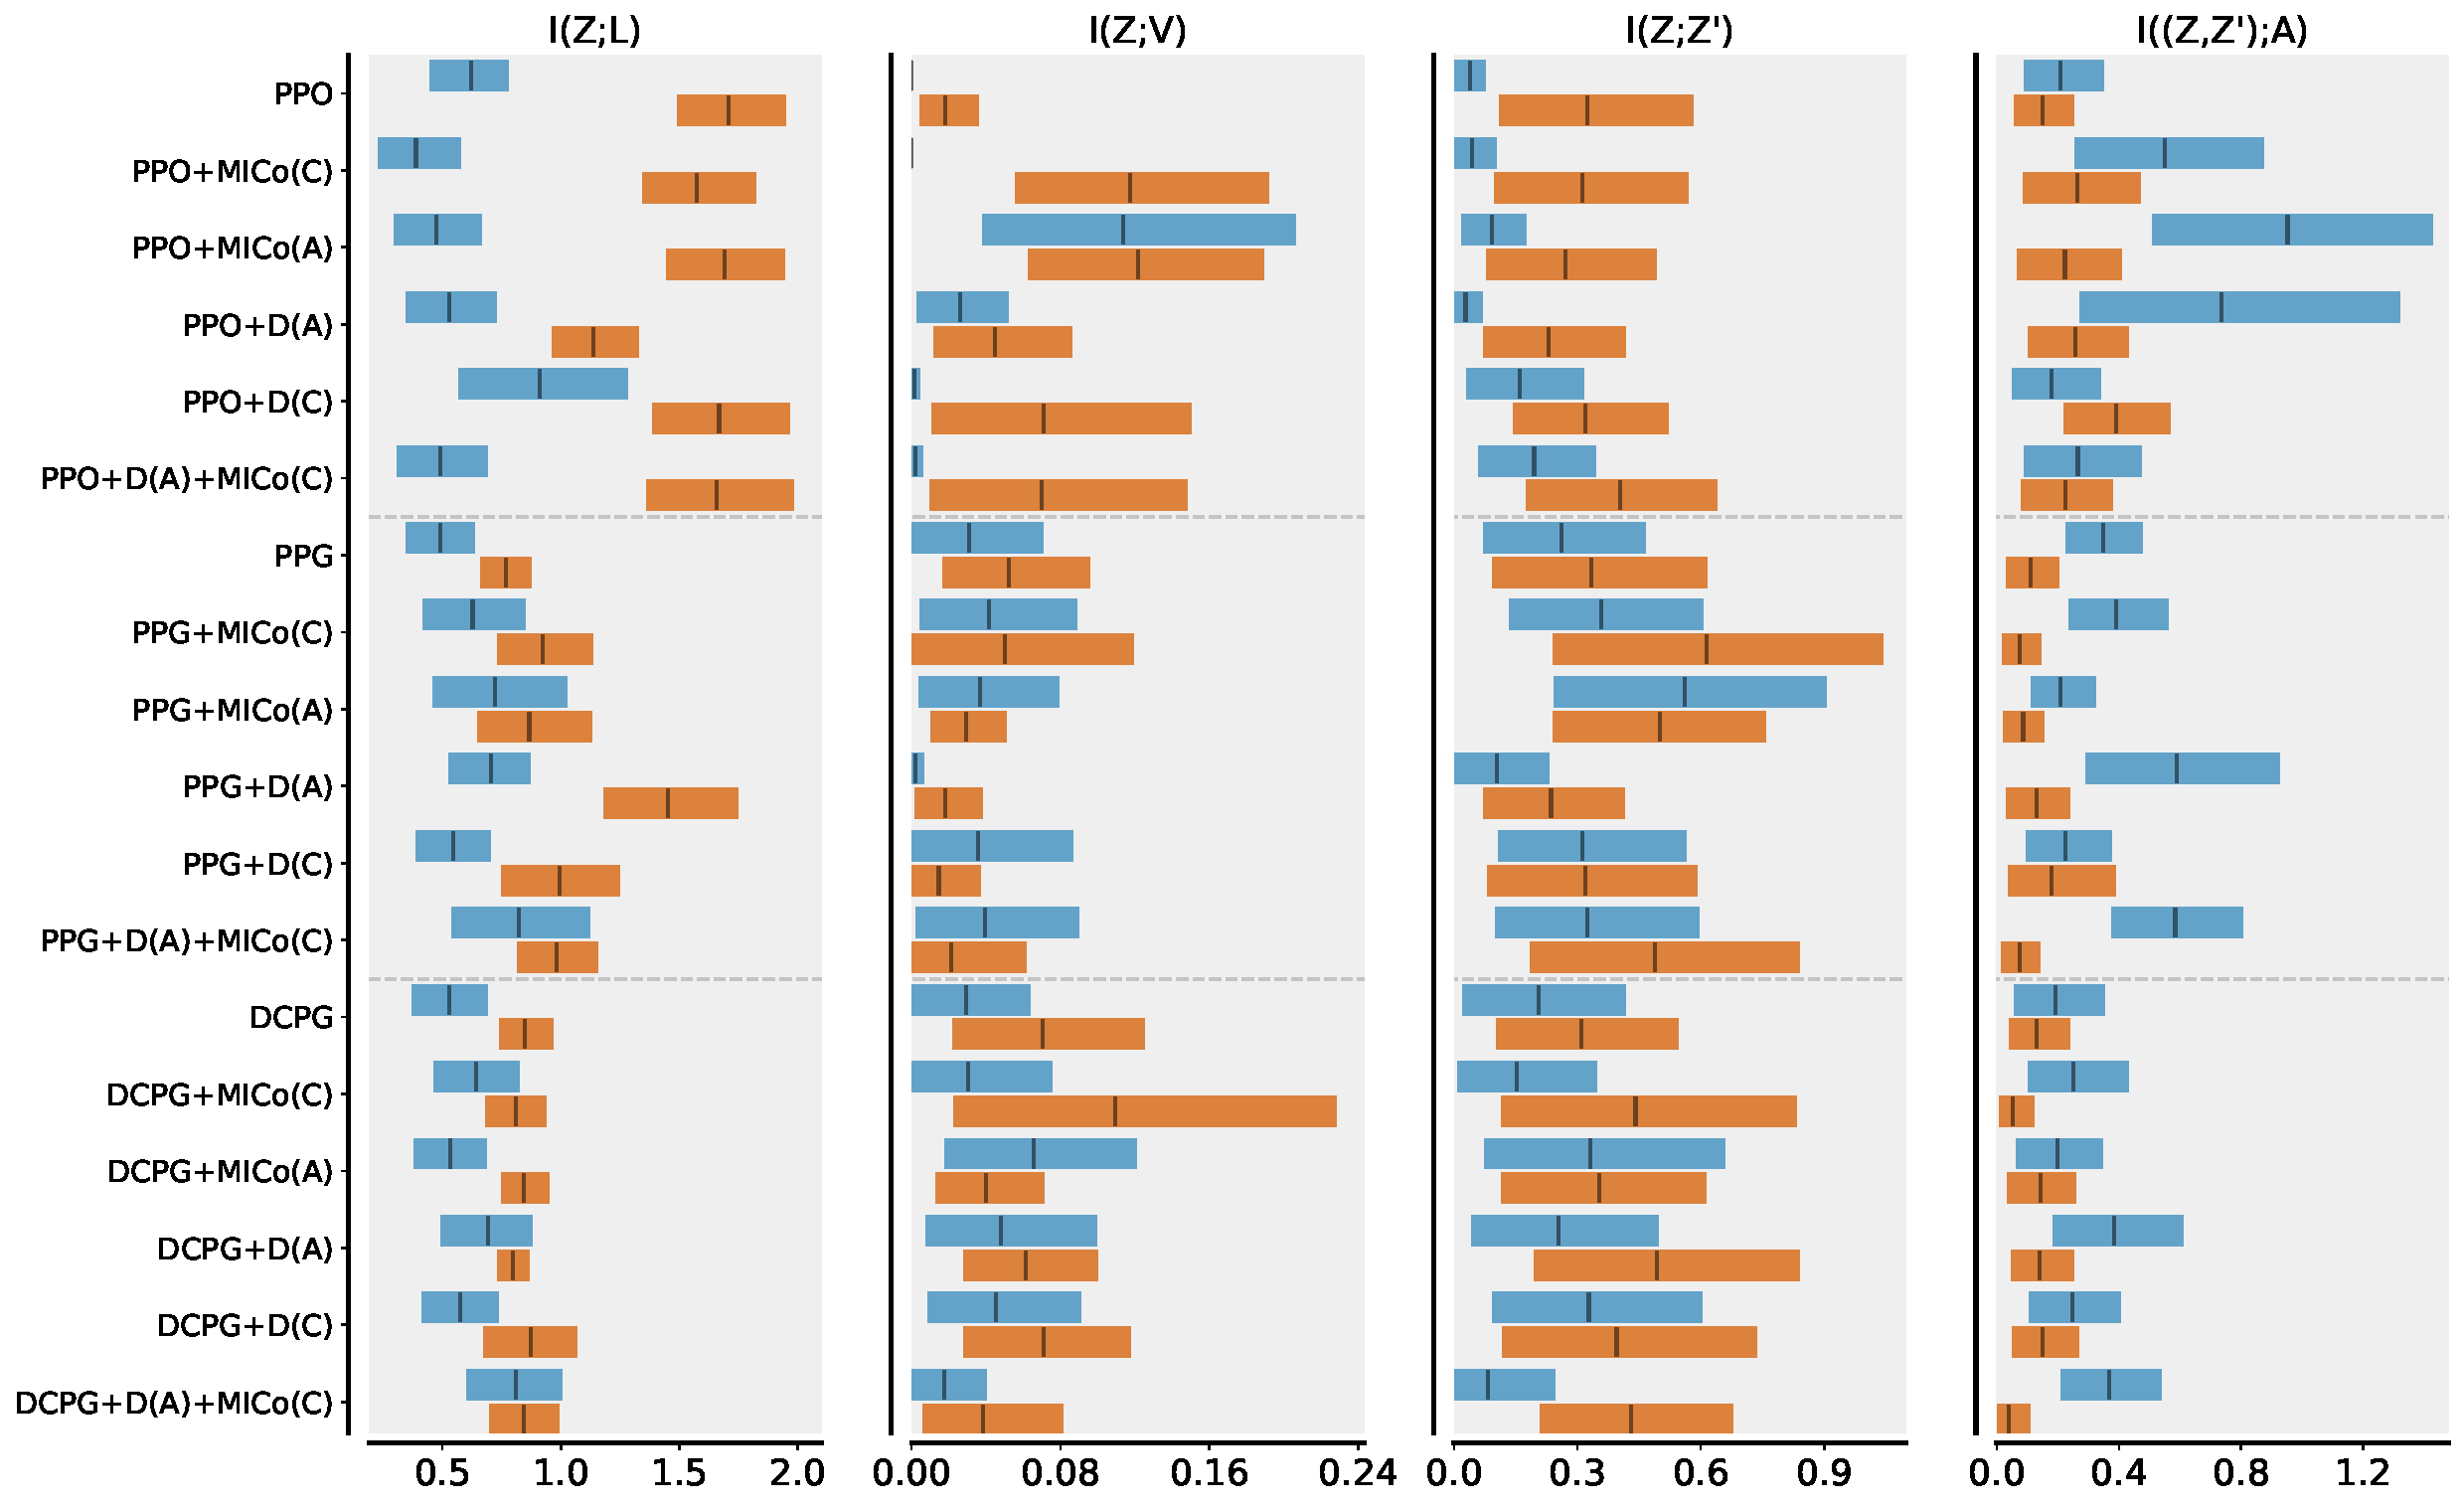
\includegraphics[width=0.97\textwidth]{figs/brax_all_algos_mi.pdf}
    \end{center}
    \caption{Mutual information measurements for the actor (blue) and critic (orange) for auxiliary losses for PPO, PPG, and DCPG in Brax.}
    \label{c2:fig:brax_all_mi}
\end{figure}

\begin{figure}[!h]
    \begin{center}
    \centering
    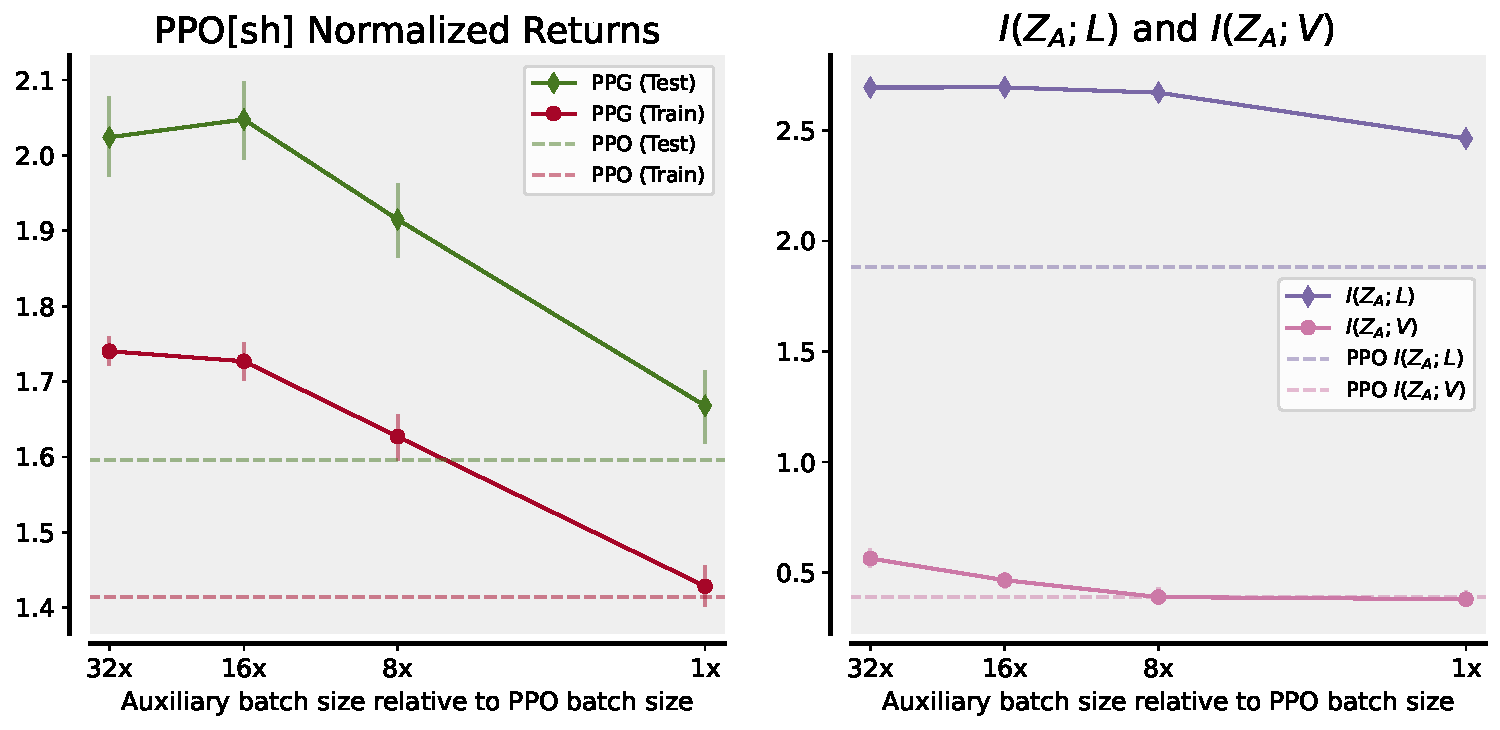
\includegraphics[width=0.97\textwidth]{figs/procgen_scaling_aux.pdf}
    \end{center}
    \caption{Procgen PPG returns (left) normalized by PPO[sh] performance and mutual information quantities $I(Z_A;L)$/$I(Z_A;V)$ (right) for varying auxiliary batch size levels.}
    \label{c2:fig:PPGvalue_dist}
\end{figure}

\begin{figure}[!h]
    \begin{center}
    \centering
    \begin{subfigure}[]{0.48\linewidth}
        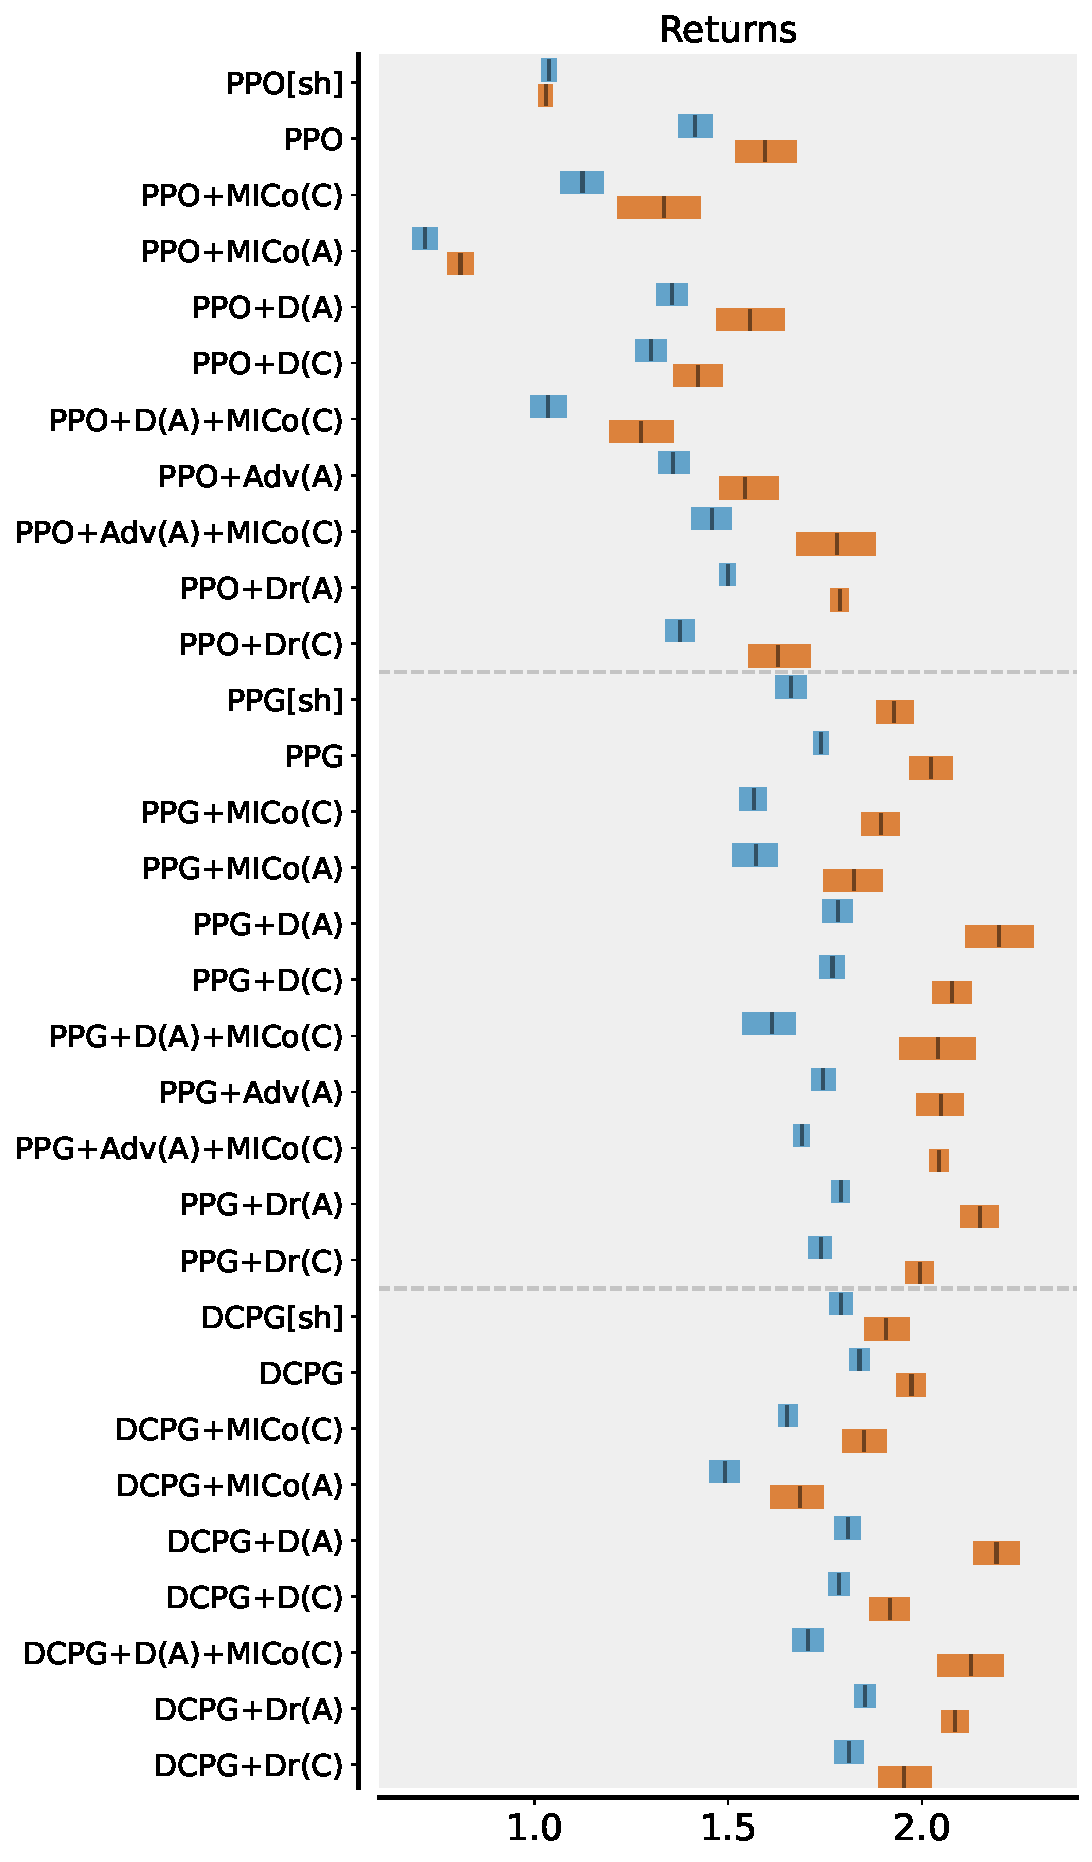
\includegraphics[width=1\linewidth]{figs/procgen_returns.pdf}
    \end{subfigure}
    \begin{subfigure}[]{0.48\linewidth}
        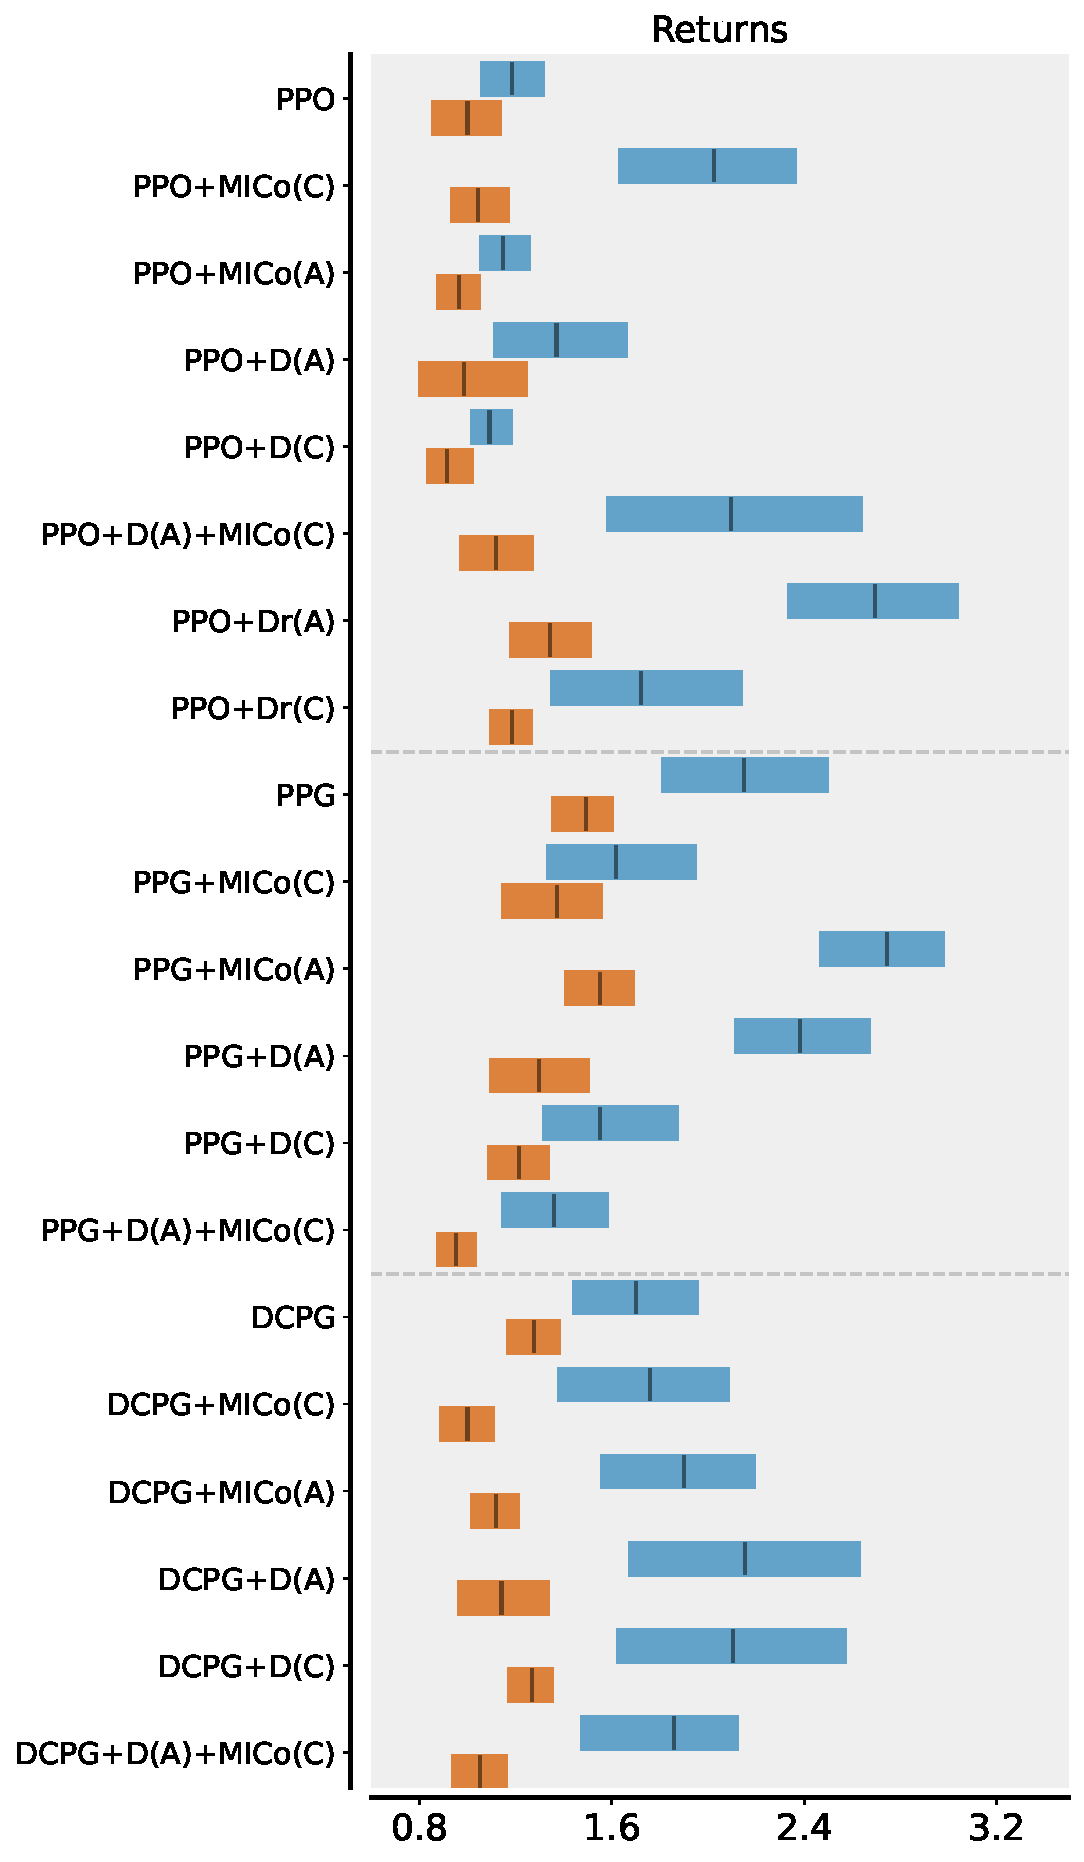
\includegraphics[width=1\linewidth]{figs/brax_returns.pdf}
    \end{subfigure}
    % \begin{subfigure}[]{0.32\linewidth}
    %     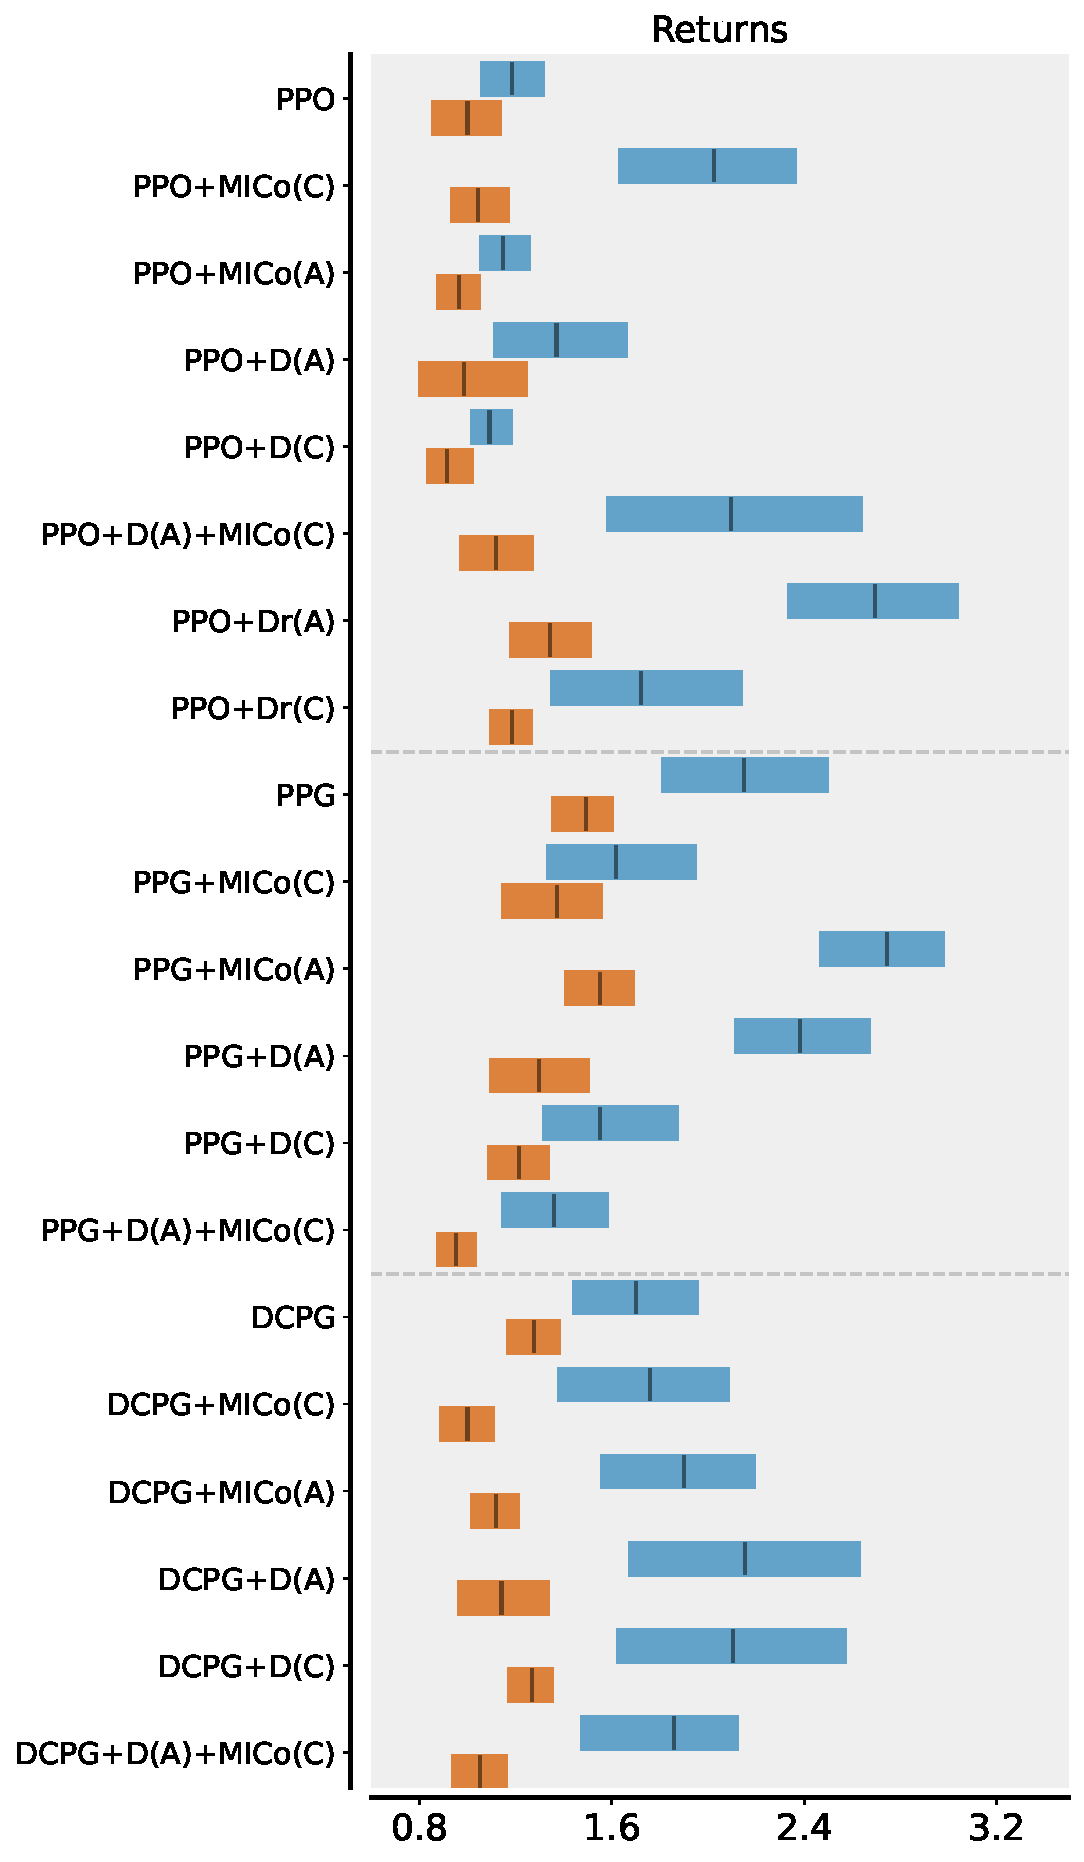
\includegraphics[width=1\linewidth]{figs/brax_returns.pdf}
    % \end{subfigure}
    \end{center}
    \caption{Returns in Procgen (left) and Brax (right).}
\label{c2:fig:complete-returns}
\end{figure}


\newpage

\begin{table}[!h]
\caption{Measurements of compression efficiency $\comp{Z_A \vert O}{V}$ (\Cref{c2:eqn:compression-eff}) with standard error in Procgen. Statistical significance bolded, determined by Welch's t-test. Results highlighted in red when decoupling decreases $\comp{Z_A \vert O}{V}$, and highlighted in green when decoupling increases $\comp{Z_A \vert O}{V}$, otherwise yellow. Coupled architectures are denoted with algorithm name plus ``[sh]''.}
\label{c2:tab:decoupled-C}
\begin{center}
\begin{tabular}{l|c|c}
\textbf{Algorithm} & $C(Z_A \vert O;V)$ & $C(Z_A \vert O;L)$
\\ \hline
PPO[sh] & 89.3 $\pm$ 2 & 65.2 $\pm$ 3 \\
PPO & \colorbox{yellow}{90.1 $\pm$ 4} & \textbf{\colorbox{pink}{52.3 $\pm$ 3}} \\ \hline
PPG[sh] & 85.9 $\pm$ 4 & 70.0 $\pm$ 2 \\
PPG & \colorbox{yellow}{94.1 $\pm$ 2} & \textbf{\colorbox{green}{75.5 $\pm$ 2}} \\ \hline
DCPG[sh] & 95.4 $\pm$ 2 & 77.6 $\pm$ 2 \\
DCPG & \colorbox{yellow}{92.3 $\pm$ 7} & \colorbox{yellow}{76.4 $\pm$ 2}
\end{tabular}
\end{center}
\end{table}

% \begin{figure}[!h]
%     \begin{center}
%     \begin{subfigure}[]{1\linewidth}
%         \center
%         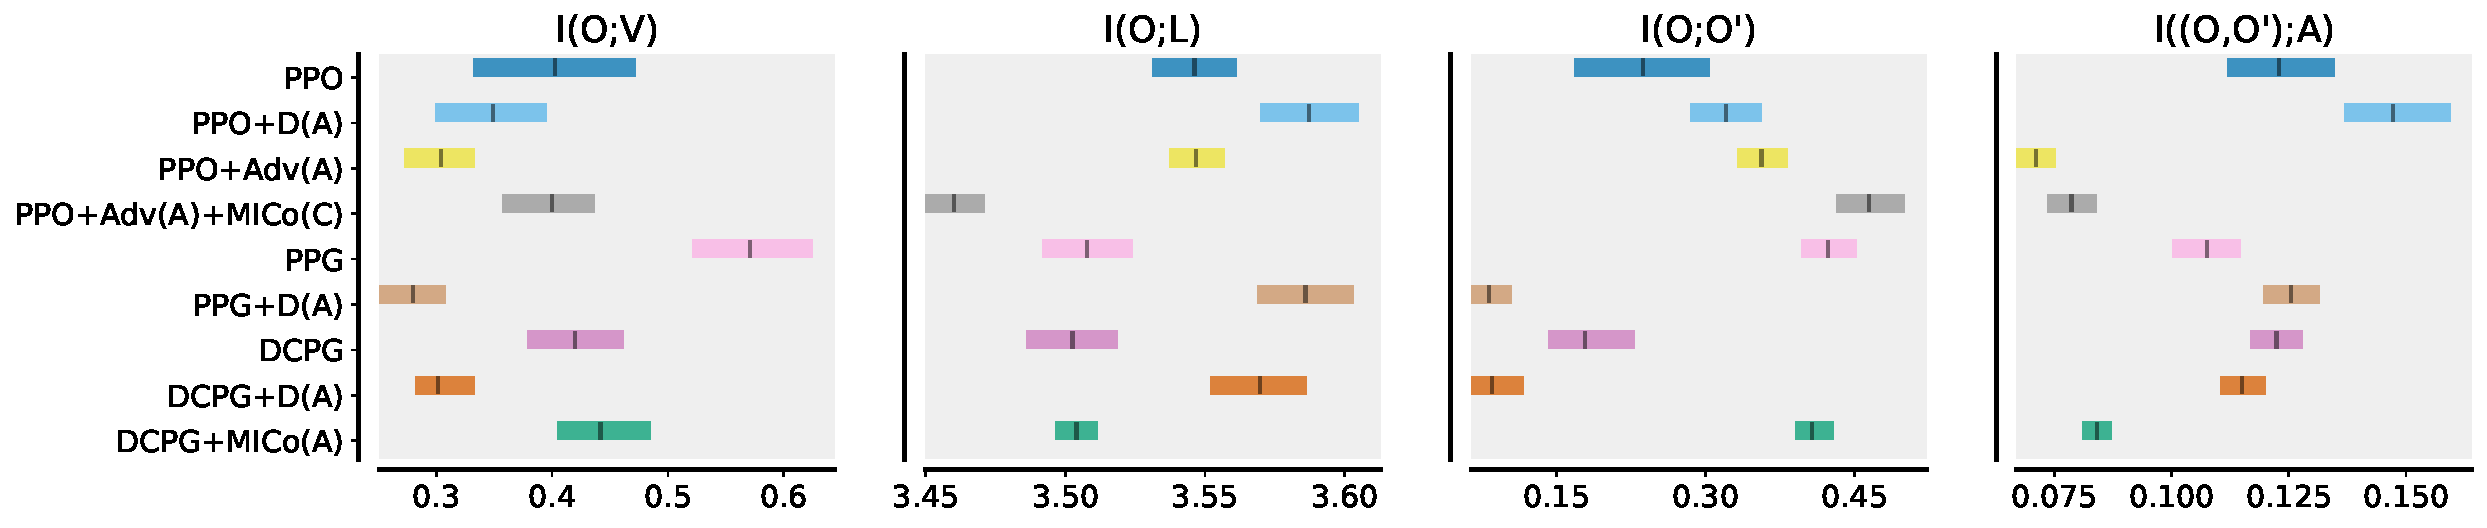
\includegraphics[width=0.9\linewidth]{figs/procgen_actor_obs.pdf}
%     \end{subfigure}
%     \begin{subfigure}[]{1\linewidth}
%         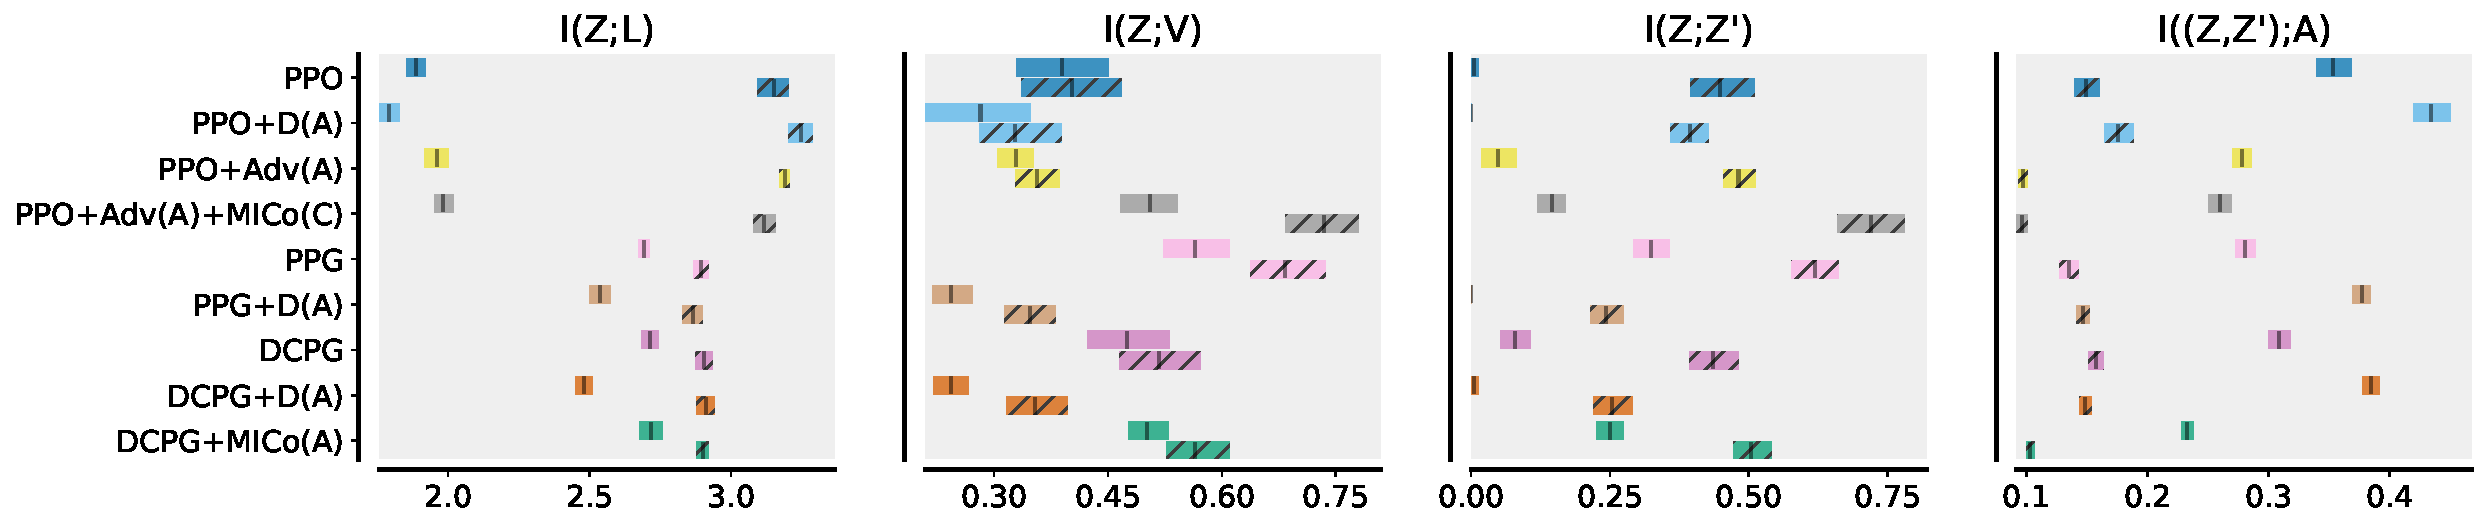
\includegraphics[width=1\linewidth]{figs/procgen_actor_obs_bottom.pdf}
%     \end{subfigure}
%     % \begin{subfigure}[]{1\linewidth}
%     %     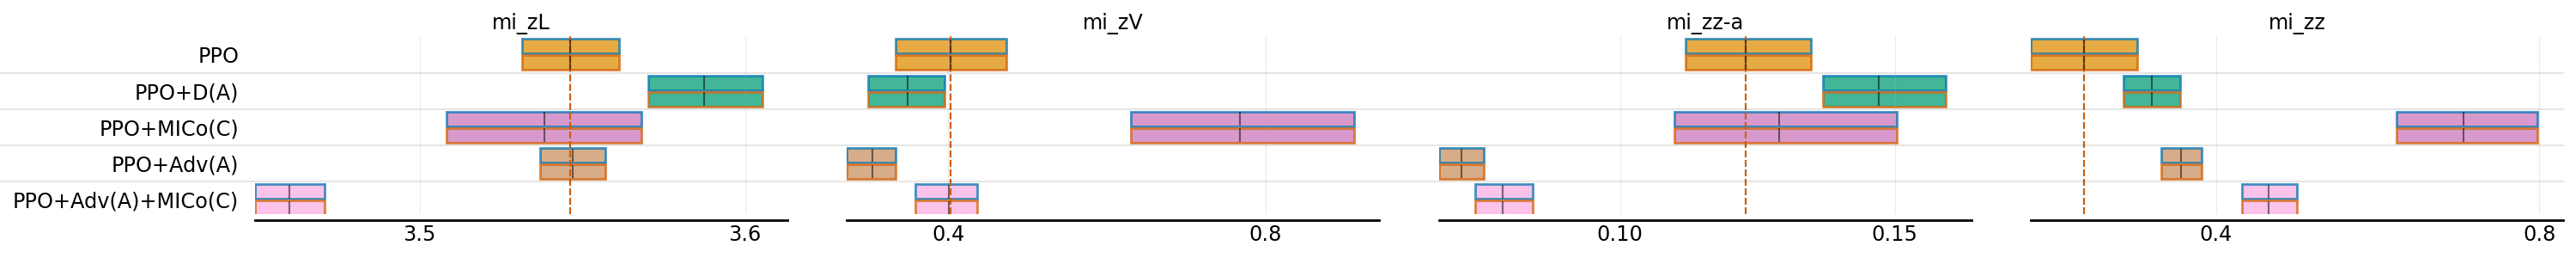
\includegraphics[width=1\linewidth]{figs/ppo_obs_train.png}
%     % \end{subfigure}
%     % \begin{subfigure}[]{1\linewidth}
%     %     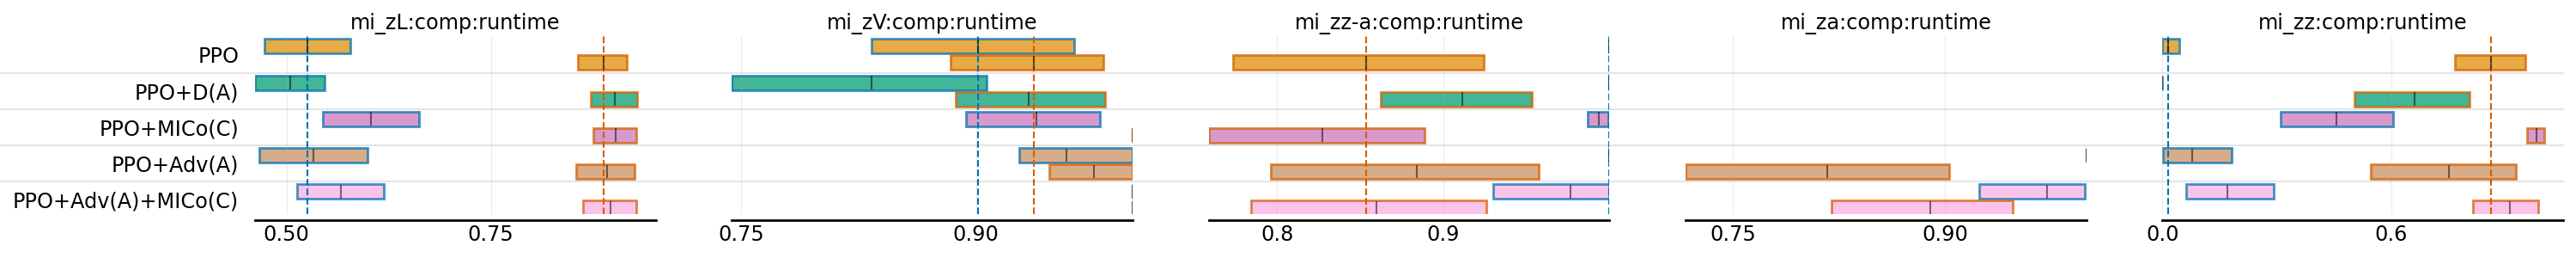
\includegraphics[width=1\linewidth]{figs/ppo_comp_train.png}
%     % \end{subfigure}
%     \end{center}
%     \caption{Mean and 95\% confidence interval of mutual information measurements for actor (non-hashed) and critic (hashed) representation for base PPO, dynamics prediction on the actor (D(A)), MICo on the critic (MICo(C)), and advantage via the actor (Adv(A)). $\mut{O}{\cdot}$ show one bar because these measurements do not involve representations produced by $\phi_A$ nor $\phi_C$.}
%     \label{c2:fig:aux-losses-actor}
%     % \todoin{Figure is cluttered and not paper ready yet. Clean up by:
%     % \begin{itemize}
%     %     \item same todos as \Cref{c2:fig:shdec-spec-obs-comp}
%     %     \item Fix mismatch between objective combinations plotted and discussed in main text.
%     % \end{itemize}}
% \end{figure}

\begin{table}[!h]
\caption{Measurements of compression efficiency $\comp{Z_A \vert O}{\cdot}$ (\Cref{c2:eqn:compression-eff}) of the actor's representation $\phi_A$ in Procgen. Results highlighted in red when the auxiliary loss decreases the metric relative to the base algorithm, and highlighted in green when the auxiliary loss increases the metric relative to the base algorithm. Auxiliary losses are applied to the actor  (A) and critic (C) in the form of dynamics prediction (D), MICo, and advantage distillation (Adv).}
\label{c2:tab:actor-C}
\begin{center}
\begin{tabular}{l|c|c|c}
\textbf{Algorithm} & $C(Z_A \vert O;V)$ & $C(Z_A \vert O;L)$ & $C((Z_A|O,Z^{\prime}_A|O^{\prime});A)$
\\ \hline
PPO & 90.1 $\pm$ 4 & 52.3 $\pm$ 3 & 99.9 $\pm$ 0 \\
PPO+MICo(C) & \colorbox{yellow}{93.9 $\pm$ 2 } & \textbf{\colorbox{green}{60.4 $\pm$ 3 }} & \colorbox{yellow}{99.4 $\pm$ 0 } \\ 
PPO+MICo(A) & \colorbox{yellow}{98.6 $\pm$ 1 } & \textbf{\colorbox{green}{84.7 $\pm$ 2 }} & \textbf{\colorbox{pink}{87.5 $\pm$ 5 }} \\ 
PPO+D(A) & \colorbox{yellow}{62.6 $\pm$ 12 } & \textbf{\colorbox{green}{61.3 $\pm$ 2 }} & \colorbox{yellow}{100.0 $\pm$ 0 } \\ 
PPO+D(C) & \colorbox{yellow}{86.8 $\pm$ 7 } & \colorbox{yellow}{52.8 $\pm$ 3 } & \colorbox{yellow}{100.0 $\pm$ 0 } \\ 
PPO+D(A)+MICo(C) & \colorbox{yellow}{76.3 $\pm$ 6 } & \textbf{\colorbox{green}{63.7 $\pm$ 3 }} & \colorbox{yellow}{99.5 $\pm$ 0 } \\ 
PPO+Adv(A) & \colorbox{yellow}{96.9 $\pm$ 2 } & \colorbox{yellow}{53.2 $\pm$ 3 } & \colorbox{yellow}{100.0 $\pm$ 0 } \\ 
PPO+Adv(A)+MICo(C) & \textbf{\colorbox{green}{100.0 $\pm$ 0 }} & \colorbox{yellow}{57.0 $\pm$ 2 } & \colorbox{yellow}{98.5 $\pm$ 1 } \\ 
PPO+Dr(A) & \colorbox{yellow}{89.1 $\pm$ 6 } & \colorbox{yellow}{54.3 $\pm$ 3 } & \colorbox{yellow}{100.0 $\pm$ 0 } \\ 
PPO+Dr(C) & \colorbox{yellow}{98.1 $\pm$ 1 } & \colorbox{yellow}{50.8 $\pm$ 3 } & \colorbox{yellow}{99.6 $\pm$ 0 } \\ \hline
PPG & 94.1 $\pm$ 2 & 75.5 $\pm$ 2 & 100.0 $\pm$ 0 \\
PPG+MICo(C) & \colorbox{yellow}{98.0 $\pm$ 1 } & \colorbox{yellow}{76.4 $\pm$ 2 } & \colorbox{yellow}{100.0 $\pm$ 0 } \\ 
PPG+MICo(A) & \colorbox{yellow}{95.4 $\pm$ 2 } & \textbf{\colorbox{green}{85.8 $\pm$ 2 }} & \colorbox{yellow}{100.0 $\pm$ 0 } \\ 
PPG+D(A) & \colorbox{yellow}{89.5 $\pm$ 4 } & \colorbox{yellow}{71.2 $\pm$ 2 } & \colorbox{yellow}{100.0 $\pm$ 0 } \\ 
PPG+D(C) & \colorbox{yellow}{96.3 $\pm$ 2 } & \colorbox{yellow}{75.1 $\pm$ 2 } & \colorbox{yellow}{100.0 $\pm$ 0 } \\ 
PPG+D(A)+MICo(C) & \colorbox{yellow}{85.9 $\pm$ 7 } & \colorbox{yellow}{71.6 $\pm$ 2 } & \colorbox{yellow}{100.0 $\pm$ 0 } \\ 
PPG+Adv(A) & \colorbox{yellow}{98.4 $\pm$ 1 } & \textbf{\colorbox{pink}{63.3 $\pm$ 2 }} & \colorbox{yellow}{100.0 $\pm$ 0 } \\ 
PPG+Adv(A)+MICo(C) & \colorbox{yellow}{99.4 $\pm$ 1 } & \textbf{\colorbox{pink}{62.9 $\pm$ 2 }} & \colorbox{yellow}{100.0 $\pm$ 0 } \\ 
PPG+Dr(A) & \colorbox{yellow}{91.3 $\pm$ 3 } & \colorbox{yellow}{74.9 $\pm$ 2 } & \colorbox{yellow}{100.0 $\pm$ 0 } \\ 
PPG+Dr(C) & \colorbox{yellow}{93.1 $\pm$ 6 } & \colorbox{yellow}{75.6 $\pm$ 2 } & \colorbox{yellow}{100.0 $\pm$ 0 } \\ \hline
DCPG & 92.3 $\pm$ 7 & 76.4 $\pm$ 2 & 100.0 $\pm$ 0 \\
DCPG+MICo(C) & \colorbox{yellow}{98.1 $\pm$ 1 } & \colorbox{yellow}{76.6 $\pm$ 2 } & \colorbox{yellow}{100.0 $\pm$ 0 } \\ 
DCPG+MICo(A) & \colorbox{yellow}{91.7 $\pm$ 3 } & \colorbox{yellow}{74.3 $\pm$ 2 } & \colorbox{yellow}{100.0 $\pm$ 0 } \\ 
DCPG+D(A) & \colorbox{yellow}{80.9 $\pm$ 4 } & \textbf{\colorbox{pink}{69.9 $\pm$ 2 }} & \colorbox{yellow}{100.0 $\pm$ 0 } \\ 
DCPG+D(C) & \colorbox{yellow}{97.8 $\pm$ 1 } & \colorbox{yellow}{76.3 $\pm$ 2 } & \colorbox{yellow}{100.0 $\pm$ 0 } \\ 
DCPG+D(A)+MICo(C) & \colorbox{yellow}{83.4 $\pm$ 5 } & \textbf{\colorbox{pink}{69.6 $\pm$ 2 }} & \colorbox{yellow}{100.0 $\pm$ 0 } \\ 
DCPG+Dr(A) & \colorbox{yellow}{97.5 $\pm$ 2 } & \colorbox{yellow}{76.7 $\pm$ 2 } & \colorbox{yellow}{100.0 $\pm$ 0 } \\ 
\end{tabular}
\end{center}
\end{table}

\begin{table}[!h]
\caption{Measurements of compression efficiency $\comp{Z_C \vert O}{\cdot}$ (\Cref{c2:eqn:compression-eff}) of the actor's representation $\phi_C$ in Procgen. Results highlighted in red when the auxiliary loss decreases the metric relative to the base algorithm, highlighted in green when the auxiliary loss increases the metric relative to the base algorithm, and highlighted in yellow otherwise. Auxiliary losses are applied to the actor  (A) and critic (C) in the form of dynamics prediction (D), MICo, and advantage distillation (Adv).}
\label{c2:tab:critic-C}
\begin{center}
\begin{tabular}{l|c|c|c}
\textbf{Algorithm} & $C(Z_C \vert O;V)$ & $C(Z_C \vert O;L)$ & $C((Z_C|O,Z^{\prime}_C | O^{\prime};A))$
\\ \hline
PPO & 93.7 $\pm$ 3 & 88.4 $\pm$ 2 & 85.6 $\pm$ 4 \\
PPO+MICo(C) & \colorbox{yellow}{100.0 $\pm$ 0 } & \colorbox{yellow}{90.3 $\pm$ 1 } & \colorbox{yellow}{82.7 $\pm$ 3 } \\ 
PPO+MICo(A) & \colorbox{yellow}{97.6 $\pm$ 2 } & \colorbox{yellow}{92.4 $\pm$ 1 } & \textbf{\colorbox{pink}{64.4 $\pm$ 6 }} \\ 
PPO+D(A) & \colorbox{yellow}{99.7 $\pm$ 0 } & \colorbox{yellow}{90.2 $\pm$ 1 } & \colorbox{yellow}{87.4 $\pm$ 3 } \\ 
PPO+D(C) & \colorbox{yellow}{87.6 $\pm$ 4 } & \textbf{\colorbox{pink}{77.4 $\pm$ 2 }} & \textbf{\colorbox{green}{99.1 $\pm$ 0 }} \\ 
PPO+D(A)+MICo(C) & \colorbox{yellow}{91.0 $\pm$ 6 } & \colorbox{yellow}{88.1 $\pm$ 2 } & \colorbox{yellow}{84.4 $\pm$ 3 } \\ 
PPO+Adv(A) & \colorbox{yellow}{96.7 $\pm$ 2 } & \colorbox{yellow}{89.3 $\pm$ 1 } & \colorbox{yellow}{87.6 $\pm$ 4 } \\ 
PPO+Adv(A)+MICo(C) & \colorbox{yellow}{100.0 $\pm$ 0 } & \colorbox{yellow}{89.9 $\pm$ 1 } & \colorbox{yellow}{87.0 $\pm$ 3 } \\ 
PPO+Dr(A) & \colorbox{yellow}{98.0 $\pm$ 1 } & \colorbox{yellow}{90.0 $\pm$ 1 } & \colorbox{yellow}{87.9 $\pm$ 3 } \\ 
PPO+Dr(C) & \colorbox{yellow}{97.5 $\pm$ 1 } & \colorbox{yellow}{87.0 $\pm$ 2 } & \colorbox{yellow}{86.3 $\pm$ 3 } \\ \hline
PPG & 99.2 $\pm$ 1 & 81.6 $\pm$ 2 & 90.3 $\pm$ 3 \\
PPG+MICo(C) & \colorbox{yellow}{93.0 $\pm$ 6 } & \textbf{\colorbox{green}{90.9 $\pm$ 2 }} & \colorbox{yellow}{91.8 $\pm$ 2 } \\ 
PPG+MICo(A) & \colorbox{yellow}{100.0 $\pm$ 0 } & \colorbox{yellow}{80.9 $\pm$ 2 } & \colorbox{yellow}{84.4 $\pm$ 4 } \\ 
PPG+D(A) & \colorbox{yellow}{100.0 $\pm$ 0 } & \colorbox{yellow}{79.2 $\pm$ 2 } & \colorbox{yellow}{91.3 $\pm$ 3 } \\ 
PPG+D(C) & \textbf{\colorbox{pink}{89.4 $\pm$ 4 }} & \colorbox{yellow}{77.6 $\pm$ 2 } & \textbf{\colorbox{green}{100.0 $\pm$ 0 }} \\ 
PPG+D(A)+MICo(C) & \colorbox{yellow}{93.3 $\pm$ 4 } & \textbf{\colorbox{green}{89.1 $\pm$ 2 }} & \colorbox{yellow}{87.1 $\pm$ 4 } \\ 
PPG+Adv(A) & \colorbox{yellow}{100.0 $\pm$ 0 } & \colorbox{yellow}{80.9 $\pm$ 2 } & \colorbox{yellow}{89.7 $\pm$ 3 } \\ 
PPG+Adv(A)+MICo(C) & \colorbox{yellow}{99.9 $\pm$ 0 } & \colorbox{yellow}{92.3 $\pm$ 1 } & \colorbox{yellow}{93.1 $\pm$ 3 } \\ 
PPG+Dr(A) & \colorbox{yellow}{98.7 $\pm$ 1 } & \colorbox{yellow}{81.7 $\pm$ 2 } & \colorbox{yellow}{90.2 $\pm$ 3 } \\ 
PPG+Dr(C) & \colorbox{yellow}{96.4 $\pm$ 3 } & \colorbox{yellow}{81.8 $\pm$ 2 } & \colorbox{yellow}{85.8 $\pm$ 4 } \\ \hline
DCPG & 99.5 $\pm$ 1 & 81.7 $\pm$ 2 & 92.1 $\pm$ 3 \\
DCPG+MICo(C) & \colorbox{yellow}{98.9 $\pm$ 1 } & \textbf{\colorbox{green}{88.6 $\pm$ 2 }} & \colorbox{yellow}{93.5 $\pm$ 2 } \\ 
DCPG+MICo(A) & \colorbox{yellow}{99.8 $\pm$ 0 } & \colorbox{yellow}{81.4 $\pm$ 2 } & \colorbox{yellow}{87.2 $\pm$ 4 } \\ 
DCPG+D(A) & \colorbox{yellow}{100.0 $\pm$ 0 } & \colorbox{yellow}{80.7 $\pm$ 2 } & \colorbox{yellow}{92.6 $\pm$ 3 } \\ 
DCPG+D(C) & \textbf{\colorbox{pink}{91.3 $\pm$ 3 }} & \colorbox{yellow}{81.2 $\pm$ 1 } & \textbf{\colorbox{green}{100.0 $\pm$ 0 }} \\ 
DCPG+D(A)+MICo(C) & \colorbox{yellow}{99.6 $\pm$ 0 } & \textbf{\colorbox{green}{87.4 $\pm$ 2 }} & \colorbox{yellow}{92.7 $\pm$ 3 } \\ 
DCPG+Dr(A) & \colorbox{yellow}{100.0 $\pm$ 0 } & \colorbox{yellow}{81.3 $\pm$ 2 } & \colorbox{yellow}{89.4 $\pm$ 3 } \\ 
DCPG+Dr(C) & \colorbox{yellow}{97.0 $\pm$ 2 } & \colorbox{yellow}{81.2 $\pm$ 2 } & \colorbox{yellow}{90.7 $\pm$ 3 } \\ 
\end{tabular}
\end{center}
\end{table}

\newpage
\clearpage
\section{Implementation details}

\subsection{Mutual Information Estimation}
We measure mutual information using the estimator proposed by \citet{kraskov2004estimating} and later extended to pairings of continuous and discrete variables by \citet{ross2014mutual}. These methods are based on performing entropy estimation using k-nearest neighbors distances. We use $k=3$ and determine nearest neighbors by measuring the Euclidian ($L_2$) distance between points. We checked measurements obtained when using different $k$ and under different metric spaces, and we found that our measurements are broadly invariant to the choice of estimator parameters.

At the end of training we collect a batch of trajectories consisting of $2^{16}$ timesteps ($2^{15}$ timesteps in Brax) from $L$. We construct $( A,O,O',Z,Z',V, L )$ from $n=4096$ timesteps yielding $( a_t, o_t, o_{t+1}, z_t, z_{t+1}, v_t, c_t)$. Subsampling is necessary to compute mutual information estimates in a reasonable time, while ensuring we sample states from most levels in $L$ and at various point of the trajectories followed by the agent in each level. Timesteps are sampled uniformly and without replacement from the batch, after having excluded:
\begin{enumerate}
    \item Odd timesteps, to ensure $O$ and $O'$ will not overlap (i.e. $O$ contains only even timesteps, and $O'$, being sampled at $t+1$, contains only odd timesteps).
    \item Timesteps corresponding to episode terminations, to ensure the pair $o_t,o_t+1$ cannot originate from different levels.
    \item Timesteps from episodes that have not terminated, to ensure we can always compute $v_t$.
\end{enumerate}

\subsection{Procgen}\label{c2:app:results_procgen}
The Procgen Benchmark is a set of 16 diverse PCG environments that echoes the gameplay variety seen in the ALE benchmark \cite{ALE}. The game levels, determined by a random seed, can differ in visual design, navigational structure, and the starting locations of entities. All Procgen environments use a common discrete 15-dimensional action space and generate $64 \times 64 \times 3$ RGB observations. A detailed description of each of the 16 environments is provided by \citet{procgen}. RL algorithms such as PPO reveal significant differences between test and training performance in all games, making Procgen a valuable tool for evaluating generalisation performance. 

We conduct our experiment on the easy setting of Procgen, which employs 200 training levels and a budget of 25M training steps, and evaluate the agent's scores on the training levels and on the full range of levels, excluding the training levels. We use the version of Procgen provided by EnvPool \citep{weng2022envpool}. Following prior work, \citep{raileanu2021UCB-DrAC,PLR,DCPG}, for each game we normalise train$/$test scores by the mean train$/$test score achieved by PPO in that game. 

For PPO, we base our implementation on the CleanRL PPO implementation \citep{huang2022cleanrl}, which reimplements the PPO agent from the original Procgen publication in JAX. We use the same ResNet policy architecture and PPO hyperparameters (identical for all games) as \citet{procgen} and reported in \Cref{c2:table:hyperparams_PPO}.

We re-implement PPG and DCPG in JAX, based on the Pytorch implementations provided by \citet{huang2022cleanrl} and \citet{DCPG}. We use the default recommended hyperparameters for each algorithms, which are reported in \Cref{c2:table:hyperparams_PPG}. We note that our PPG implementation ends up outperforming the original implementation by about 10\% on the test set, while our DCPG implementation underperforms test scores reported by \citet{DCPG} by about 10\%. %It leads to DCPG achieving a mean test score 2\% lower than PPG, in both the coupled and decoupled setups. In contrast, \citet{DCPG} report that DCPG improved over PPG by 15\%. 
We attribute this discrepancy to minor differences between the JAX and Pytorch libraries, and decided to not investigate further. 

We conduct our experiments on A100 and RTX8000 Nvidia GPUs and 6 CPU cores. One seed for one game completes in 2 to 12 hours, depending on the GPU, algorithm, and whether the architecture is coupled or decoupled (for example, PPG decoupled can be expected to run 4x to 6x slower than PPO coupled).


\begin{table}[!htb]
\caption{Hyperparameters used for PPO in Procgen and Brax experiments. All runs employing a specific (or combination of) representation learning objective use the same hyperparameters.}
\label{c2:table:hyperparams_PPO}
\begin{center}
\scalebox{0.88}{
\begin{tabular}{lcccc}
\toprule
\textbf{Parameter} & Procgen & Brax\\
\midrule
\emph{PPO} & \\
$\gamma$ &0.999 & 0.999 \\
$\lambda_{\text{GAE}}$ & 0.95 & 0.95  \\
rollout length & 256 & 128 \\
minibatches per epoch & 8 & 8 \\
minibatch size & 2048 & 512\\
$J_\pi$ clip range & 0.2 & 0.2 \\
number of environments & 64 & 32 \\
Adam learning rate & 5e-4 & 5e-4 \\
Adam $\epsilon$ & 1e-5 & 1e-8  \\
max gradient norm & 0.5  & 0.5  \\
value clipping & no  & no \\
return normalisation & yes & no \\
value loss coefficient & 0.5 & 0.5 \\
entropy coefficient &  0.01  & 0.01 \\

\addlinespace[10pt]
\emph{PPO (coupled)} & & & \\
PPO epochs (actor and critic) & 3 & - \\

\addlinespace[10pt]
\emph{PPO (decoupled)} & & & \\
Actor epochs & 1 & 1 \\
Critic epochs & 9 & 1 \\

\addlinespace[10pt]
\emph{MICo objective} & & \\
MICo coefficient & 0.5 & 0.01 \\
Target network update coefficient & 0.005 & 0.05 \\

\addlinespace[10pt]
\emph{Dynamics objective} & & & \\
Dynamics loss coefficient & 1.0 & 0.01 \\
In-distribution transitions weighting & 1.0 & 1.0 \\
Out-of-distribution states weighting & 1.0 & 1.0 \\
Out-of-distribution actions weighting & 0.5 & 0.5 \\

\addlinespace[10pt]
\emph{Advantage distillation objective} & & & \\
Advantage prediction coefficient & 0.25 & - \\

\bottomrule 
\end{tabular}
}
\end{center}
\end{table}

\subsection{Brax}
For our experiments in Brax, we implement a custom ``video distractors'' set of tasks, similar to those from~\citep{DistractingDM}. In this setup, a video plays in an overlay on the pixels the agent views. There is a disjoint set of videos between the training and testing environments. The random seed determines the environment's initial physics and the video overlay at the beginning of training. The pixels themselves are full-RGB $64\times64\times3$ arrays, but we use framestacking to bring each agent input to $64\times64\times9$ pixels.

Similar to the algorithms used in the Procgen experiments, we implement our algorithms in JAX and base them on ClearnRL.

We conduct our experiments on RTX A4500 Nvidia GPUs and 6 CPU cores. One seed completes in 7.5-48 hours, depending on the environment and its physics backend as well as the algorithm.

\begin{table}[!htb]
\caption{Hyperparameters used for PPG and DCPG in Procgen experiments. Hyperparameters shared between methods are only reported if they change from the method above. All runs employing a specific (or combination of) representation learning objective use the same hyperparameters.} 
\label{c2:table:hyperparams_PPG}
\begin{center}
\scalebox{0.88}{
\begin{tabular}{lccc}
\toprule
\textbf{Parameter} & Procgen\\
\midrule
\emph{PPG} & \\
$\gamma$ &0.999  \\
$\lambda_{\text{GAE}}$ & 0.95 \\
rollout length & 256  \\ 
minibatches per epoch policy phase & 8  \\
minibatch size policy phase & 2048\\
minibatches per epoch auxiliary phase & 512  \\
minibatch size auxiliary phase & 1024\\
$J_\pi$ clip range & 0.2  \\
number of environments & 64  \\
Adam learning rate & 5e-4  \\
Adam $\epsilon$ & 1e-5  \\
max gradient norm & 0.5  \\
value clipping & no \\
return normalisation & yes \\
value loss coefficient policy phase & 0.5\\
value loss coefficient auxiliary phase & 1.0\\
entropy coefficient &  0.01  \\
policy phase epochs & 1 \\
auxiliary phase epochs & 6 \\
number of policy phases per auxiliary phase & 32 \\
policy regularisation coefficient $\beta_c$ & 1.0 \\
auxiliary value distillation coefficient & 1.0 \\

\addlinespace[10pt]
\emph{DCPG} &   \\
value loss coefficient policy phase & 0.0\\
delayed value loss coefficient policy phase & 1.0\\

\addlinespace[10pt]
\emph{MICo objective} & \\
MICo coefficient & 0.5 \\
Target network update coefficient & 0.005 \\

\addlinespace[10pt]
\emph{Dynamics objective} & & & \\
Dynamics loss coefficient & 1.0  \\
In-distribution transitions weighting & 1.0  \\
Out-of-distribution states weighting & 1.0  \\
Out-of-distribution actions weighting & 0.5\\

\bottomrule 
\end{tabular}
}
\end{center}
\end{table}